\documentclass[12pt,english,spanish,noprefix,refpage]{book}
\usepackage{lmodern}
\renewcommand{\sfdefault}{lmss}
\renewcommand{\ttdefault}{lmtt}
\renewcommand{\familydefault}{\sfdefault}
\usepackage[T1]{fontenc}
\usepackage[latin9]{inputenc}
\usepackage{geometry}
\geometry{verbose,tmargin=2cm,bmargin=2cm,lmargin=2.5cm,rmargin=2cm}
\setcounter{secnumdepth}{3}
\setcounter{tocdepth}{3}
\usepackage{calc}
\usepackage{textcomp}
\usepackage{csquotes}
\usepackage{booktabs}
\usepackage{pgfgantt}
\usepackage{array}
\usepackage{wrapfig}
\usepackage{tabularx}
\usepackage{graphicx}
\usepackage{titlesec}
\usepackage{setspace}
\usepackage[authoryear]{natbib}
\usepackage{nomencl}
% the following is useful when we have the old nomencl.sty package
\providecommand{\printnomenclature}{\printglossary}
\providecommand{\makenomenclature}{\makeglossary}
\makenomenclature
\onehalfspacing
\definecolor{barblue}{RGB}{153,204,254}
\definecolor{groupblue}{RGB}{51,102,254}
\definecolor{linkred}{RGB}{165,0,33}
\makeatletter
\raggedbottom
\graphicspath{ {./img/} }
\title{Desarrollo de un playground para formaci�n en tecnolog�as de la Web Sem�ntica}
\author{Miguel Exp�sito Mart�n}
\let\thetitle\@title
\titleformat{\chapter}[display]   
{\normalfont\huge\bfseries}{\chaptertitlename\ \thechapter}{20pt}{\Huge}   
\titlespacing*{\chapter}{0pt}{-10pt}{30pt}
\newenvironment{changemargin}[2]{%
	\begin{list}{}{%
			\setlength{\topsep}{0pt}%
			\setlength{\leftmargin}{#1}%
			\setlength{\rightmargin}{#2}%
			\setlength{\listparindent}{\parindent}%
			\setlength{\itemindent}{\parindent}%
			\setlength{\parsep}{\parskip}%
		}%
		\item[]}{\end{list}}
\renewcommand{\footnotesize}{\scriptsize}
\setlength{\skip\footins}{1cm}
%%%%%%%%%%%%%%%%%%%%%%%%%%%%%% LyX specific LaTeX commands.
%% Because html converters don't know tabularnewline
\providecommand{\tabularnewline}{\\}

%%%%%%%%%%%%%%%%%%%%%%%%%%%%%% User specified LaTeX commands.
\usepackage{algorithmic}
\usepackage{algorithm}
\floatname{algorithm}{Algoritmo}
\usepackage{layout}
\floatname{table}{Tabla}
\usepackage{url}
\usepackage{hyperref}
\usepackage{fancyhdr}
\fancyhf{}
\setlength{\headheight}{15.2pt}
\pagestyle{fancy}
\renewcommand{\chaptermark}[1]{\markboth{#1}{}}
\makeatletter
\let\sv@endpart\@endpart
\def\@endpart{\thispagestyle{empty}\sv@endpart}
\makeatother

\makeatother

\usepackage{babel}
\addto\shorthandsspanish{\spanishdeactivate{~<>}}

\usepackage{listings}
\addto\captionsenglish{\renewcommand{\lstlistingname}{Listing}}
\addto\captionsspanish{\renewcommand{\lstlistingname}{Listado de c�digo}}
\renewcommand{\lstlistingname}{Listado de c�digo}

\begin{document}
\begin{titlepage}\thispagestyle{empty}%
\fbox{\begin{minipage}[c][0.99\textheight][t]{0.95\columnwidth}%
\vspace{1cm}
\begin{center}

\includegraphics[width=2cm]{figs/escudo_uned}
\par\end{center}
\bigskip{}
\begin{singlespace}
\begin{center}
{\large{}UNIVERSIDAD NACIONAL DE EDUCACI�N A DISTANCIA}\vspace{0.7cm}
\par\end{center}
\begin{center}
{\large{}ESCUELA T�CNICA SUPERIOR DE INGENIER�A INFORM�TICA}\vspace{0.5cm}
\par\end{center}
\begin{center}
Proyecto de Fin de Grado en Ingenier�a en Tecnolog�as de la Informaci�n {\Large{}\vspace{0.8cm}
}
\par\end{center}{\Large \par}
\end{singlespace}
\begin{center}
\textbf{\Large{}RDFplay: UN PLAYGROUND }\\
\textbf{\Large{}PARA FORMACI�N EN TECNOLOG�AS}\\
\textbf{\Large{}DE LA WEB SEM�NTICA}
\par\end{center}{\Large \par}
\vfill{}
\begin{flushleft}
\qquad{}MIGUEL EXP�SITO MART�N\bigskip{}
\par\end{flushleft}
\begin{flushleft}
\qquad{}Dirigido por: JOS� LUIS FERN�NDEZ VINDEL
\par\end{flushleft}
\begin{flushleft}
\qquad{}Co-dirigido por: RAFAEL MART�NEZ TOM�S
\par\end{flushleft}
\begin{flushleft}
\vspace{1.5cm}
\par\end{flushleft}
\begin{flushleft}
\qquad{}Curso: 2017-2018: 2� Convocatoria
\par\end{flushleft}
\bigskip{}
%
\end{minipage}}

\end{titlepage}
\thispagestyle{empty}

\cleardoublepage{}

\thispagestyle{empty}%
\fbox{\begin{minipage}[c][0.99\textheight][t]{0.95\columnwidth}%
\begin{center}
\vspace{1cm}
\par\end{center}
\begin{center}

\includegraphics[width=2cm]{figs/escudo_uned}
\par\end{center}
%\bigskip{}
\begin{singlespace}
\begin{center}
\textbf{\Large{}DESARROLLO DE UN PLAYGROUND }\\
\textbf{\Large{}PARA FORMACI�N EN TECNOLOG�AS}\\
\textbf{\Large{}DE LA WEB SEM�NTICA}
\par\end{center}{\large \par}
\end{singlespace}
\begin{center}
Proyecto de Fin de Grado de modalidad oferta espec�fica
\par\end{center}
\begin{flushleft}
\vspace{0.3cm}
\par\end{flushleft}
\begin{flushleft}
\enskip{}Realizado por:{\large{}\hspace{0.5em}}Miguel Exp�sito Mart�n{\large{}}
\vspace{0.3cm}
\par\end{flushleft}
\begin{flushleft}
\enskip{}Dirigido por:{\large{}\hspace{0.5em}}Jos� Luis Fern�ndez Vindel
\par\end{flushleft}
\begin{flushleft}
\enskip{}Co-dirigido por:{\large{}\hspace{0.5em}}Rafael Mart�nez Tom�s
\par\end{flushleft}
\begin{flushleft}
{\large{}}\vspace{0.6cm}
\par\end{flushleft}
\begin{flushleft}
\enskip{}Tribunal calificador
\par\end{flushleft}
\begin{flushleft}
\enskip{}Presidente: D/D�. 
\par\end{flushleft}
\begin{flushleft}
\textbf{\medskip{}
}
\par\end{flushleft}
\noindent \begin{flushleft}
\enskip{}Secretario: D/D�. 
\par\end{flushleft}
\begin{flushleft}
\textbf{\medskip{}
}
\par\end{flushleft}
\noindent \begin{flushleft}
\enskip{}Vocal: D/D�. 
\par\end{flushleft}
\vfill{}
\begin{flushleft}
\enskip{}Fecha de lectura y defensa: 2/10/2018
\par\end{flushleft}
\begin{flushleft}
\enskip{}Calificaci�n: 
\par\end{flushleft}
\smallskip{}
%
\end{minipage}}
\thispagestyle{empty}


\chapter*{Agradecimientos}
\begin{center}
\thispagestyle{empty}
\par\end{center}

A mi familia, a mis amigos, a mi Director de proyecto y a los que, sin querer, me animaron a afrontar este reto.


\thispagestyle{empty}

\cleardoublepage{}

\pagenumbering{roman}\fancyhead[LE,RO]{\thepage}\fancyhead[LO]{\nouppercase{\leftmark}}\fancyhead[RE]{\nouppercase{\rightmark}}\noindent \begin{center}
\textbf{\Large{}Resumen}
\par\end{center}{\Large \par}
\setlength{\parskip}{\baselineskip}
\thispagestyle{empty}

El presente proyecto tiene como objeto el desarrollo de un sistema de \textit{playground} para SPARQL y RDF que habr� de servir como herramienta educativa de introducci�n a las tecnolog�as de la Web Sem�ntica. Su prop�sito es facilitar una interfaz de uso sencilla para que usuarios profanos puedan introducirse en este tipo de tecnolog�as a un nivel b�sico, permitiendo la realizaci�n de actividades acad�micas sobre manejo sencillo de grafos as� como sobre consultas SPARQL al conjunto de datos de trabajo o a \textit{endpoints} externos.

Si bien es cierto que la Web Sem�ntica alcanza hoy en d�a un estado de madurez razonablemente avanzado, el ritmo de cambio de las tecnolog�as de \textit{frontend} en \textit{Javascript} (en adelante, JS) es, cuanto menos, vertiginoso. Unido a ello, se tiene que la mayor parte de las implementaciones de componentes de la Web Sem�ntica han sido desarrolladas en tecnolog�as de \textit{backend} como \textit{Java} (\textit{Apache Jena}) o \textit{Python} (\textit{rdflib}), no existiendo a�n est�ndares o implementaciones maduras puramente en Javascript.

Se abordan, por tanto, tres retos: la necesidad de conseguir un producto sencillo y f�cilmente utilizable por usuarios no expertos, la dificultad para encontrar componentes maduros que a�nen Web Sem�ntica con \textit{frontend} y la conveniencia de apostar por un \textit{framework} de desarrollo en \textit{Javascript} estable y con una curva de aprendizaje suave.

Para dar soluci�n a estos problemas, se ha optado por desarrollar una  \textit{Single Page Application} (SPA) con Vue.js (un \textit{framework} JS que se jacta de aglutinar las mejores caracter�sticas de Angular y React, sus principales competidores en el mercado) e integrarlo con las implementaciones recomendadas por el grupo de trabajo de bibliotecas \textit{Javascript} \textit{rdfjs} y con una plataforma de consultas para la web flexible y modular. El sistema est� planteado para ejecutarse en un sencillo navegador contempor�neo, descarg�ndose a trav�s de un simple servidor web (siendo este la �nica infraestructura necesaria para su distribuci�n).

Dado el alto nivel de incertidumbre existente a la hora de implementar las necesidades del proyecto, se ha optado por utilizar un enfoque metodol�gico incremental e iterativo basado en \textit{Extreme Programming} y apoyado sobre tableros Kanban, lo que ha permitido una mejor organizaci�n y evoluci�n del proyecto.

El resultado final ofrece un producto b�sico de introducci�n a las tecnolog�as de la Web Sem�ntica y permite pensar en un desarrollo del mismo tan ambicioso como las propias necesidades de los equipos docentes, dado el estado de madurez actual del \textit{frontend} web.\thispagestyle{empty}

\selectlanguage{english}%
\noindent \begin{center}
\textbf{\Large{}Abstract}
\par\end{center}{\Large \par}

\noindent \thispagestyle{empty}

<This project ...>\selectlanguage{spanish}%

\thispagestyle{empty}

\cleardoublepage{}

\tableofcontents{}\cleardoublepage{}\markboth{\nomname}{\nomname}

\printnomenclature{}

\listoffigures

\renewcommand{\listtablename}{�ndice de tablas} 

\listoftables

\cleardoublepage{}
\fancyhf{}
\pagenumbering{arabic}
\pagestyle{fancy}
\fancyhead[LE,RO]{\thepage}
\fancyhead[LO]{\chaptername {} \thechapter. \leftmark}
\fancyhead[RE]{\slshape Desarrollo de un playground para formaci�n en tecnolog�as de la Web Sem�ntica}

\chapter{Introducci�n}

No cabe duda que uno de los retos a los que se enfrenta la Sociedad de la Informaci�n y del Conocimiento es la educaci�n, una de las mejores inversiones en el futuro de Europa. Seg�n la �ltima Comunicaci�n de la Comisi�n al Parlamento, al Consejo, al Comit� Econ�mico y Social Europeo y al Comit� de las Regiones\cite{comission01},  el uso de las TIC para prop�sitos educativos se queda atr�s, tanto en adopci�n como en competencias del profesorado. La innovaci�n en sistemas educativos, entendida como la adopci�n de nuevos servicios y herramientas por parte de las organizaciones educativas, puede mejorar los resultados formativos y la eficiencia.

Siendo una de las prioridades del Plan de Acci�n propuesto por la Comisi�n hacer mejor uso de la tecnolog�a digital para el aprendizaje y la ense�anza, parece apropiado que instituciones como la Universidad Nacional de Educaci�n a Distancia (UNED) en Espa�a y sus departamentos, como el de Inteligencia Artificial, se propongan aplicar los �ltimos avances tecnol�gicos para mejorar la calidad del sistema educativo y facilitar a los alumnos la adquisici�n de nuevas competencias digitales complejas.

Dentro de estas competencias se pueden encuadrar t�rminos como Web de Datos, Web Sem�ntica o Datos Enlazados, todos definidos por el padre de la Web, Tim Berners-Lee\cite{bernerslee01, bernerslee02}. No son m�s que la evoluci�n l�gica de la Web a la que todos estamos acostumbrados, pero entendida en su crecimiento como una soluci�n a los problemas de la ingente cantidad de datos no estructurados o inconexos que se genera al d�a en 2018 (seg�n Domo\cite{domo01}, 2,5 quintillones de bytes).
 
En concreto, este trabajo pretende acercar las tecnolog�as de la Web Sem�ntica al alumnado siguiendo las recomendaciones del  W3C RDFJS Community Group\cite{rdfw3ccg} a trav�s de una sencilla aplicaci�n puramente desarrollada en Javascript y lista para usar, que permita la exploraci�n de facilidades de modelado y consulta sobre un conjunto de datos predefinido o aportado por el propio alumno as� como la carga y realizaci�n de actividades simples propuestas por el profesorado.


La memoria de este proyecto se estructura en los siguientes cap�tulos:

\begin{itemize}
	\item \textbf{Cap�tulo 1. Introducci�n.}  Esta introducci�n.
	\item \textbf{Cap�tulo 2. La Web Sem�ntica.} Una presentaci�n de las tecnolog�as que conforman la Web Sem�ntica: datos enlazados, RDF y SPARQL.
	\item \textbf{Cap�tulo 3. Motivaci�n y objetivos.} Se exponen las razones que llevaron a la elecci�n de este proyecto en concreto, as� como las metas que se esperaban alcanzar.
	\item \textbf{Cap�tulo 4. Trabajos previos, estado actual y recursos.} Un estudio sobre el estado actual de las tecnolog�as en cuesti�n y los recursos que se estiman necesarios para llevar a cabo con �xito el proyecto.
	\item \textbf{Cap�tulo 5. Metodolog�a y planificaci�n.} Descripci�n de la metodolog�a de desarrollo de software a utilizar y an�lisis de las planificaciones llevada a cabo (inicial y efectiva).
	\item \textbf{Cap�tulo 6. An�lisis.} Se presenta un estudio de necesidades para el sistema de informaci�n concretadas en casos de uso detallados.
	\item \textbf{Cap�tulo 7. Dise�o.} Descripci�n de las distintas arquitecturas del sistema, as� como su estructura basada en componentes.
	\item \textbf{Cap�tulo 8. Implementaci�n y pruebas.} Detalles de implementaci�n en Javascript y de las pruebas unitarias y extremo a extremo llevadas a cabo.
	\item \textbf{Cap�tulo 9. Resultados.}
	\item \textbf{Cap�tulo 10. Conclusiones y l�neas futuras de trabajo.}
\end{itemize}\cleardoublepage{}

\chapter{La Web Sem�ntica}

Cabe comenzar el desarrollo de la presente memoria con una breve introducci�n a los fundamentos de la Web Sem�ntica y las tecnolog�as que la sustentan: RDF y SPARQL. Asimismo, queda definido tambi�n el t�rmino de datos enlazados o \textit{linked data}, estrechamente relacionado con estos conceptos y de gran importancia hoy en d�a en la difusi�n de datos estructurados a trav�s de Internet.

\section{Fundamentos}

La Web Sem�ntica es un t�rmino originalmente acu�ado por Tim Berners-Lee en el a�o 2001\cite{bernerslee01}. Hasta la fecha, la \textit{World Wide Web} hab�a sido concebida como una idea de colaboraci�n abierta en la que m�ltiples contribuciones de varios autores pod�an tener cabida y ser compartidas universalmente. Dichas contribuciones, realizadas en forma de documentos, estaban dirigidas a personas y no a m�quinas o computadores. Berners-Lee vio m�s all� y propuso su extensi�n para lograr su manipulaci�n autom�tica; en resumidas cuentas, permitir que agentes inteligentes (programas de ordenador) fueran capaces de encontrar datos y su significado a trav�s de hiperenlaces a definiciones de t�rminos clave y reglas de razonamiento e inferencia l�gica.

Para lograr tan ambicioso objetivo, los agentes inteligentes necesitar�an tener acceso a contenido y conocimiento estructurado, as� como a las reglas de inferencia necesarias. En este contexto, la Web Sem�ntica pod�a apoyarse en las siguientes tecnolog�as ya existentes:

\begin{itemize}  
	\item  \textbf{RDF} (\textit{Resource Description Framework}), que permite expresar conocimiento en forma de tripletas o ternas (a modo de sujeto, verbo y objeto en una oraci�n) utilizando URIs (\textit{Uniform Resource Indicators}\footnote{Cadenas de caracteres que identifican los recursos de una red de forma un�voca.}).
	\item \textbf{XML} (\textit{eXtensible Markup Language}), un metalenguaje que permite crear lenguajes de etiquetado o marcado y documentos a su vez convenientemente etiquetados y con estructura arbitraria.
\end{itemize}

Sin embargo, un tercer pilar era necesario para resolver la problem�tica de la existencia de distintos identificadores en distintas bases de datos relacionadas con el mismo significado conceptual. Gracias a las \textbf{ontolog�as}, documentos que definen formalmente las relaciones entre distintos t�rminos, estas diferencias pod�an ser salvadas bien mediante el uso de t�rminos estandarizados bien mediante la definici�n de relaciones conceptuales de igualdad o similitud entre dichos t�rminos.

En palabras del propio Berners-Lee: \blockquote[{\cite{bernerslee01}}]{Con un dise�o adecuado, la Web Sem�ntica puede ayudar en la evoluci�n del conocimiento humano como un todo.}

\section{Linked Data}

Estrechamente relacionado con la Web Sem�ntica se encuentra el concepto de datos enlazados o \textit{Linked Data}, tambi�n propuesto por Berners-Lee en 2006\cite{bernerslee02} en lo que se considera como su introducci�n oficial y formal. Se trata de un movimiento respaldado por el propio W3C que se centra en conectar conjuntos de datos a lo largo de la Web y que puede verse como un subconjunto de la Web Sem�ntica.

Se basa, por tanto, en dos aspectos clave:

\begin{itemize}
	\item La publicaci�n de conjuntos datos estructurados en l�nea.
	\item El establecimiento de enlaces entre dichos conjuntos de datos.
\end{itemize}

La Web Sem�ntica es el fin y los datos enlazados proporcionan el medio para alcanzar dicho fin.

\section{RDF}

Las tecnolog�as de la Web Sem�ntica permiten, por tanto, almacenar conocimiento en forma de conceptos y relaciones a trav�s de ternas o tripletas, modelar dominios de conocimiento con vocabularios est�ndar y ofrecer potentes facilidades de consulta sobre dichos modelos. Dentro de estas tecnolog�as, RDF es, sin duda, el bloque de construcci�n fundamental en la Web Sem�ntica (como HTML lo ha sido para la Web).

RDF fue propuesto por el W3C en 1999\cite{Lassila:99:RDF} como un est�ndar para crear y procesar metadatos con el objetivo de describir recursos independientemente de su dominio de aplicaci�n, ayudando por tanto a promover la interoperabilidad entre aplicaciones.

Sin embargo, con la llegada de la Web Sem�ntica el alcance de RDF creci�, y ya no s�lo se usa para codificar metadatos sobre recursos web, sino tambi�n \textbf{para describir cualquier recurso as� como sus relaciones} en el mundo real.

El nuevo alcance de RDF qued� reflejado en las especificaciones publicadas en 2004 por el \textit{RDF Core Working Group}\footnote{Recomendaciones del W3C, https://www.w3.org/2001/sw/RDFCore/}, ahora actualizadas a fecha de 2014\footnote{Versiones actualizadas de las recomendaciones del W3C, https://www.w3.org/2011/rdf-wg/wiki/Main\_Page}, de las que se pueden extraer las siguientes definiciones de RDF:


\vspace*{\baselineskip}
\begin{center}
	\begin{table}[htb]
		\centering
		\begin{tabular}{p{3cm}p{10cm}}
			\toprule
			Recomendaci�n & Definici�n \\ \midrule
			RDF Primer & Un marco de trabajo para expresar informaci�n sobre recursos. \\ \midrule
			RDF Concepts \& Syntax & Un marco de trabajo para representar informaci�n en la Web. \\ 
			\bottomrule
		\end{tabular}
		\caption{Definiciones de RDF en las recomendaciones del W3C}
		\label{tabdefrdf}
	\end{table}
\end{center}

\subsection{Modelo Abstracto de RDF}

RDF ofrece un modelo abstracto que permite descomponer el conocimiento en peque�as piezas llamadas sentencias (\textit{statements}), tripletas o ternas y que toman la forma:

\begin{center}
Sujeto - Predicado - Objeto
\end{center}

En donde \textit{Sujeto} y \textit{Objeto} representan dos conceptos o ``cosas'' en el mundo (tambi�n denominados \textbf{recursos}) y \textit{Predicado} la relaci�n que los conecta.

Los nombres de estos recursos (as� como de los predicados) han de ser globales y deber�an identificarse por un \textit{Uniform Resource Idenfifier} (URI).

Por tanto, un modelo RDF puede expresarse como una colecci�n de tripletas o un grafo, dado que estas no son m�s que grafos dirigidos. Los sujetos y objetos ser�an los nodos del grafo y los predicados sus aristas.

Otra nomenclatura utilizada para representar una terna ser�a la siguiente:

\begin{center}
	Recurso - Propiedad - Valor de la propiedad
\end{center}

En donde el valor de la propiedad u Objeto tambi�n puede ser un literal, que consiste simplemente en un dato textual bruto.

Cabe destacar que una terna RDF s�lo puede modelar relaciones binarias. Para modelar una relaci�n n-aria, suelen utilizarse recursos intermedios como nodos en blanco, que no son m�s que sujetos u objetos que no tienen un URI como identificador (nodos sin nombre o an�nimos).

En resumen:

\vspace*{\baselineskip}
\begin{center}
	\begin{table}[htb]
		\centering
		\begin{tabular}{p{5cm}p{6cm}}
			\toprule
			Sujeto & Puede ser un URI o un nodo en blanco. \\ \midrule
			Predicado o Propiedad & Debe ser un URI. \\ \midrule
			Objeto o Valor de la Propiedad & Puede ser un URI, un literal o un nodo en blanco. \\
			\bottomrule
		\end{tabular}
		\caption{Resumen conceptual de ternas}
		\label{tabresterna}
	\end{table}
\end{center}

\pagebreak

A continuaci�n se muestran dos ejemplos de tripletas:

\vspace*{\baselineskip}
\begin{center}
	\begin{table}[htb]
		\tiny
		\centering
		\begin{tabular}{p{5cm}p{5cm}p{5cm}}
			\toprule
			Sujeto & Predicado & Objeto \\ \midrule
			http://www.uned.es/ia/example\#Analista & http://www.w3.org/1999/02/22-rdf-syntax-ns\#type & http://www.w3.org/2002/07/owl\#Class  \\ \midrule
		    http://www.uned.es/ia/example\#Analista & http://www.w3.org/2000/01/rdf-schema\#label & ``Analista Inform�tico'' \\ 
			\bottomrule
		\end{tabular}
		\caption{Ejemplos de tripletas reales}
		\label{tabejternas}
	\end{table}
\end{center}

\subsection{Aplicaciones pr�cticas de RDF}

Gracias a RDF, es posible construir la Web Sem�ntica y enlazar conjuntos de datos. A continuaci�n se enumeran algunas de sus aplicaciones reales:

\begin{itemize}  
	\item A�adir informaci�n legible a los motores de b�squeda.
	\item Enriquecer un conjunto de datos enlaz�ndolo con conjuntos de datos de terceros.
	\item Facilitar el descubrimiento de APIs\footnote{\textit{Aplication Programming Interface}, en este caso referido a puntos accesibles a trav�s de la Web.} a trav�s de su entrelazado.
	\item Construir agregaciones de datos sobre determinados temas.
	\item Proporcionar un est�ndar de intercambio de datos entre bases de datos.
	\item Enriquecer, describir y contextualizar los datos mediante un enfoque rico en metadatos.
\end{itemize}

Su principal ventaja frente a los modelos y bases de datos relacionales es una mayor facilidad para evolucionar los grafos, algo que en un sistema relacional es complejo (dado que requiere de modificaciones en las estructuras de almacenamiento de datos y sus consultas asociadas). En otras palabras, su \textbf{flexibilidad para modelar lo inesperado}.

Un ejemplo claro a nivel global es Wikidata\footnote{https://www.wikidata.org/wiki/Wikidata:Main\_Page}, una base de datos de conocimiento abierta que puede ser le�da y editada tanto por personas como por m�quinas. Wikidata act�a como un almac�n centralizado para datos estructurados de otros proyectos hermanos como Wikipedia, Wikisource, etc. En el momento de redacci�n de esta memoria, cuenta con  50,035,140 elementos de datos que cualquiera puede editar.
 
De una forma m�s concreta, es destacable el importante rol de RDF y las tecnolog�as de la Web Sem�ntica en �mbitos de \textbf{b�squeda y clasificaci�n bibliogr�fica o documental}, pudiendo citarse como ejemplo la publicaci�n en RDF del \textit{Diccionario de Lugares Geogr�ficos} y el \textit{Diccionario y Tesauro de Materias} del Patrimonio Cultural de Espa�a, gestionado en la actualidad por el Ministerio de Educaci�n, Cultura y Deporte del Gobierno de Espa�a\footnote{https://www.mecd.gob.es/cultura-mecd/areas-cultura/museos/destacados/2015/tesauros.html}.

\section{SPARQL} \label{sec:sparql}

Tal y como SQL provee (al menos, relativamente) un de un est�ndar de consulta  para las bases de datos relacionales, SPARQL ofrece un lenguaje de consulta estandarizado para grafos RDF. 

SPARQL es un acr�nimo recursivo para \textit{SPARQL Protocol And RDF Query Language}; es a la vez un lenguaje de consulta de grafos RDF y un protocolo, dado que permite exponer servicios web que acepten consultas en dicho lenguaje.

Entre sus caracter�sticas, cabe citar:

\begin{itemize}  
	\item Recuperaci�n de valores de datos estructurados o semi-estructurados.
	\item Exploraci�n de conjuntos de datos a trav�s de consultas sobre relaciones desconocidas.
	\item Ejecuci�n de uniones complejas sobre bases de datos dispersas en una �nica consulta.
	\item Transformaci�n de datos RDF desde un vocabulario a otro.
\end{itemize}

\pagebreak

La estructura b�sica de una consulta SPARQL es la siguiente:

\begin{lstlisting}[basicstyle=\tiny, caption={Estructura b�sica de consulta SPARQL.},captionpos=b]

# declaraciones de prefijos
PREFIX foo: <http://example.com/resources/>
...
# definici�n del conjunto de datos
FROM ...
# cl�usula de resultado
SELECT ...
# patr�n de la consulta
WHERE {
	...
}
# modificadores de la consulta
ORDER BY ...
\end{lstlisting} 

No es objeto de este proyecto profundizar en la sintaxis del lenguaje, pero s� se incluye a continuaci�n un ejemplo de consulta:

\begin{lstlisting}[basicstyle=\tiny, caption={Consulta que devuelve todos los nombres de personas mencionadas en un grafo.},captionpos=b]
PREFIX foaf:  <http://xmlns.com/foaf/0.1/>
SELECT ?name
WHERE {
	?person foaf:name ?name .
}
\end{lstlisting} 

\cleardoublepage{}

\chapter{Motivaci�n y objetivos}

Conocer los motivos que impulsan a llevar a cabo una determinada acci�n facilita la empat�a entre seres humanos, promueve el contagio de ilusiones y ayuda a comprender. El presente cap�tulo cuenta con dos secciones bien diferenciadas, explicando la motivaci�n que llev� a la elecci�n de este proyecto y los objetivos que se intentaban conseguir con el mismo.

\section{Motivaci�n}

En el �mbito acad�mico, la Web Sem�ntica se contextualiza e integra en materias como la \textit{Gesti�n Avanzada de la Informaci�n y el Conocimiento}, donde las Tecnolog�as de la Informaci�n se insertan con la Inteligencia Artificial con el objeto de modelar conocimiento humano para un posterior procesamiento y aprendizaje autom�tico.

Las tecnolog�as de la Web Sem�ntica se caracterizan por un cambio de paradigma bastante brusco con respecto a otras tecnolog�as de manipulaci�n de datos con las que un alumno muy probablemente pueda estar familiarizado a la hora de introducirse en este nuevo mundo. Es cierto que pueden establecerse ciertas comparativas conceptuales para facilitar su comprensi�n; como ejemplo, el cuadro \ref{comprelsem} equipara la Web Sem�ntica con un sistema basado en bases de datos relacionales.

\vspace*{\baselineskip}
\begin{center}
	\begin{table}[htb]
		\centering
		\begin{tabular}{p{5cm}p{5cm}}
			\toprule
			Mundo Relacional & Mundo Sem�ntico \\ \midrule
		    Registro de tabla & Nodo \gls{RDF} \\ \midrule
		    Columna de tabla & \gls{RDF} propertyType \\ \midrule
			Celda de tabla & Valor \\ \midrule
			Consulta \gls{SQL} & Consulta \gls{SPARQL} \\ \midrule
			Modelo de datos & Ontolog�a \\ 
			\bottomrule
		\end{tabular}
		\caption{Comparativa paradigma relacional vs sem�ntico.}
		\label{comprelsem}
	\end{table}
\end{center}

\pagebreak

Sin embargo, determinados indicadores pueden dar lugar a entender que la interiorizaci�n de los conceptos asociados a la Web Sem�ntica no es sencilla. Por ejemplo: su uso casi exclusivamente acad�mico con poca penetraci�n en el mundo empresarial, su lenta velocidad de propagaci�n, su soporte limitado en determinadas plataformas tecnol�gicas o incluso el t�mido inter�s mostrado en el �mbito p�blico (excluyendo honrosas excepciones como el acad�mico o universitario, las iniciativas de datos abiertos o lo relativo a la biblioteconom�a). Un ejemplo muy concreto, real y tangible de esta escasa penetraci�n es el reducido n�mero de art�culos (cuatro) presentado en \textit{workshops} como \textit{SemStats}\footnote{\textit{SemStats} es un \textit{workshop} de celebraci�n anual centrado en el estado actual de las tecnolog�as de la Web Sem�ntica aplicadas a la estad�stica p�blica. Ver \url{http://semstats.org/}}\cite{semstats2018}, de cuyo \textit{Program Comittee} este autor forma parte:


\begin{figure}[h]
	\centering
	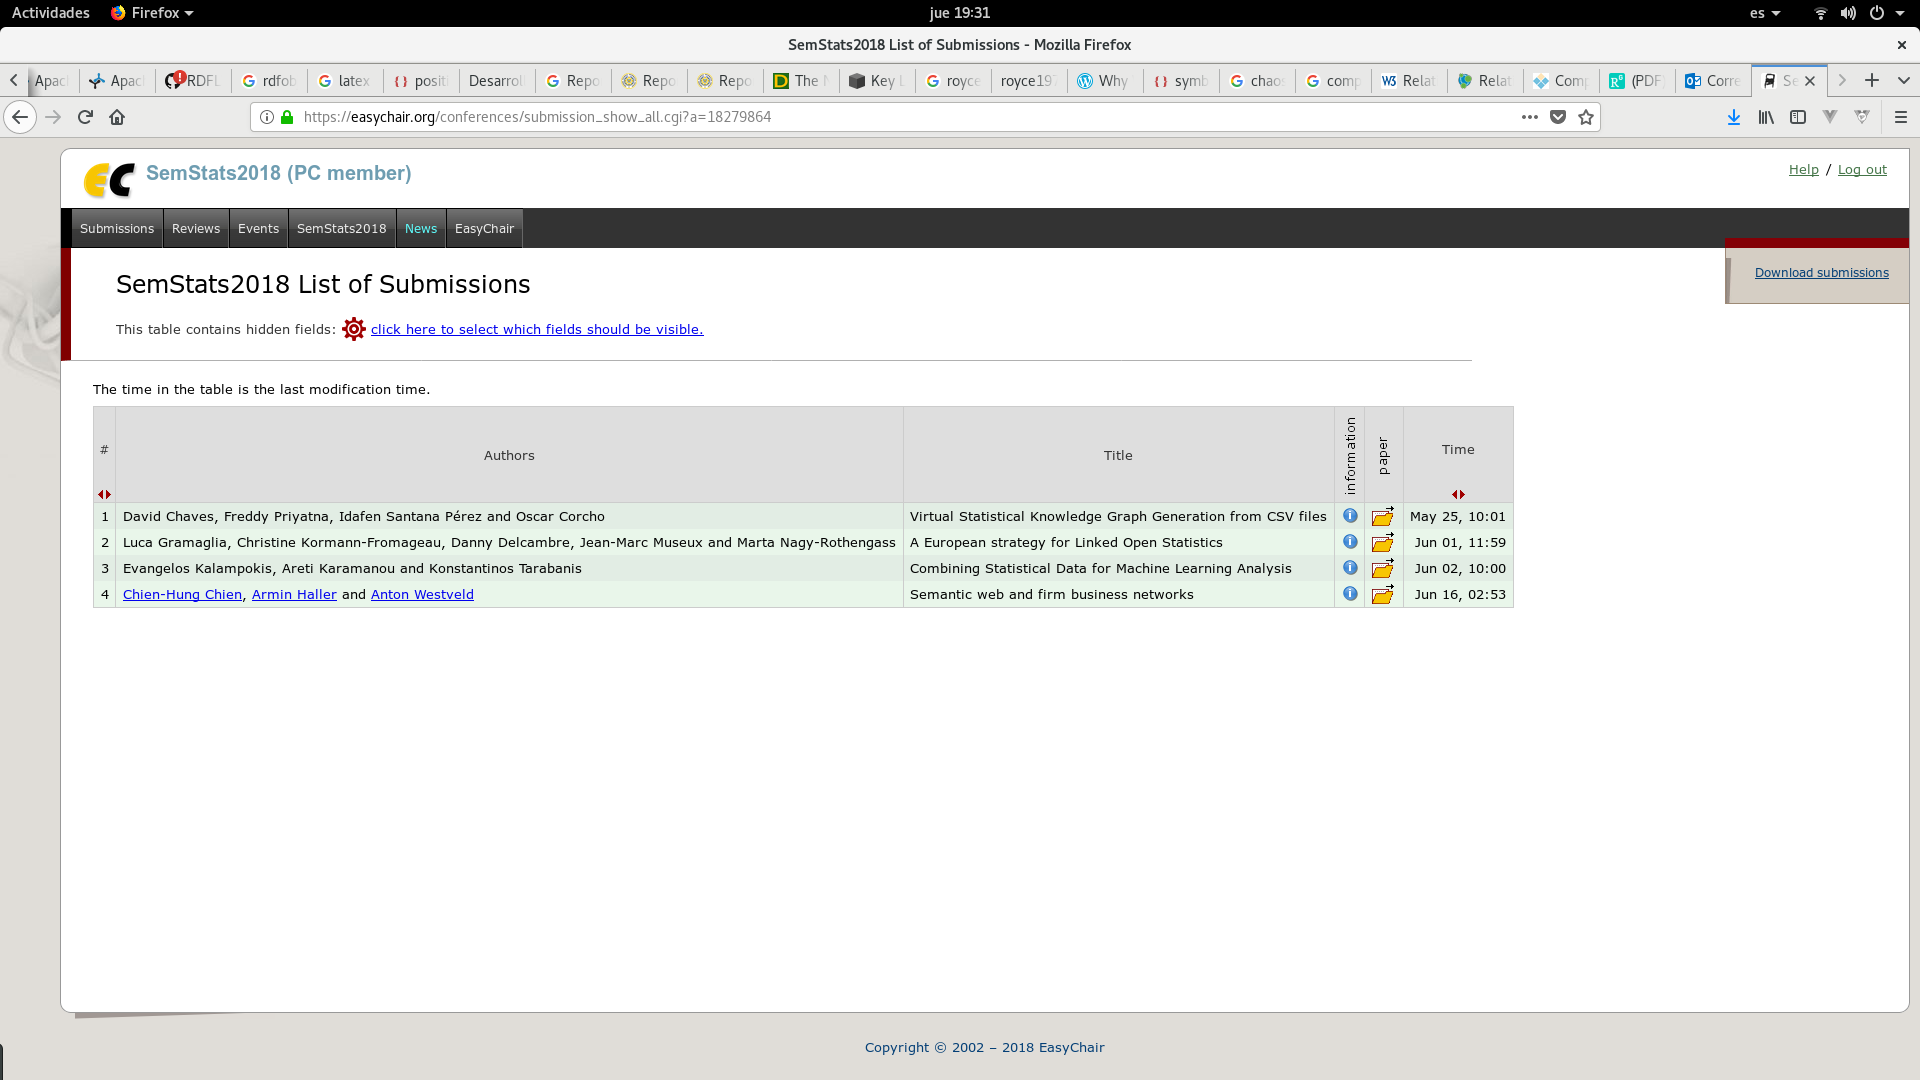
\includegraphics[scale=0.25]{semstats2018}
	\caption{Trabajos enviados a \textit{Semstats} 2018.}
\end{figure}

En este caso, resulta cuando menos sorprendente que las Oficinas Estad�sticas P�blicas, encargadas de generar y publicar datos estad�sticos sobre econom�a, poblaci�n y sociedad en general, no est�n mostrando mayor inter�s a la hora no ya de publicar sus datos en formatos enlazables, sino de construir aplicaciones sem�nticas para explotar y relacionar mejor estos datos.

Es esta \textbf{situaci�n de dificultad en el aprendizaje y en la interiorizaci�n de la utilidad de las tecnolog�as de la Web Sem�ntica la que motiva}, en �ltima instancia, la idea de desarrollar herramientas que acerquen este tipo de tecnolog�as al p�blico en general y faciliten una toma de contacto gradual con las mismas, ayudando as� a su divulgaci�n. 

\section{Objetivos} \label{objetivos}

Si bien es cierto que existen, por una parte, varias aproximaciones gratuitas en la red a modo de \textit{playground} que permiten el lanzamiento de consultas \gls{SPARQL} a determinados \textit{endpoints} y por otra, editores y herramientas de modelado del calibre de \textit{Prot�g�}\footnote{\label{protegefn}Un editor de ontolog�as y marco de trabajo para construir sistemas inteligentes. Ver \url{https://protege.stanford.edu/}} (analizados con detalle en la secci�n \ref{trabajosprevios}), no parece haber en el mercado referencias de aplicaciones que ofrezcan simult�neamente subconjuntos reducidos de ambas funcionalidades. Llenar este hueco y \textbf{conseguir una herramienta formativa �nica de modelado y consulta en tecnolog�as de la Web Sem�ntica }que permita a los equipos docentes de las asignaturas relacionadas con tecnolog�as de la Web Sem�ntica ofrecer a los alumnos (o a cualquier no iniciado en estas tecnolog�as) un \textit{playground} o entorno de pruebas que les ayude a consolidar su aprendizaje te�rico con una base pr�ctica adaptada al mundo real \textbf{es el objetivo principal de este proyecto}.

De forma m�s espec�fica, es posible enumerar los siguientes objetivos detallados:

\begin{enumerate}  
	\item  Facilitar el aprendizaje y la \textbf{familiarizaci�n con tecnolog�as de la Web Sem�ntica} a usuarios inexpertos.
	\item Reducir al m�ximo los requisitos de uso de la herramienta para alcanzar el mayor p�blico objetivo posible.
	\item Ofrecer a los equipos docentes la posibilidad de \textbf{distribuir actividades formativas} auto-contenidas para que los alumnos trabajen sobre ellas en la herramienta.
	\item Agrupar en un solo producto \textbf{funcionalidades b�sicas de edici�n y consulta sobre grafos \gls{RDF}}, de cara a cubrir las expectativas educativas en este �mbito.
	\item Permitir a los alumnos comprobar \textit{in situ} los efectos de sus acciones sobre un grafo \gls{RDF} y ofrecerles la \textbf{flexibilidad suficiente} como para permitirles dar rienda suelta a su creatividad e inquietudes.
	
	Y por �ltimo, y no menos importante, 
	
	\item \textbf{Obtener un \gls{MVP}}\footnote{Un producto con las suficientes caracter�sticas como para satisfacer a sus usuarios tempranos.} que pueda ser evolucionado y poner su c�digo a disposici�n de la comunidad educativa para revertir sobre ella su valor aportado.
\end{enumerate}
\cleardoublepage{}


\chapter{Trabajos previos, estado actual y recursos}


\section{Trabajos previos} \label{trabajosprevios}

Para enfocar el presente proyecto se llev� a cabo un estudio previo de los trabajos existentes que pudieran estar relacionado con los objetivos del mismo. En las siguientes subsecciones se analizan las familias de herramientas analizadas.

\subsection{Herramientas de consulta}

La herramienta de consulta web que se asemeja m�s a los resultados obtenidos con este proyecto es el SPARQL playground desarrollado por el \textit{Swiss Institute of Bioinformatics}\footnote{https://www.isb-sib.ch}.

Se trata de una aplicaci�n web\textit{ standalone} y multiplataforma cuyo prop�sito fundamental es el aprendizaje de SPARQL. Sus autores proporcionan una demo \textit{online}\footnote{http://sparql-playground.sib.swiss/} adem�s de documentaci�n y consultas de ejemplo para que cualquiera pueda familiarizarse con este lenguaje de consulta.

Si bien sus funcionalidades de consulta son muy completas, carece de facilidades de edici�n de grafos propios o de consulta a \textit{endpoints} externos, por ejemplo.

\begin{figure}[h]
	\centering
	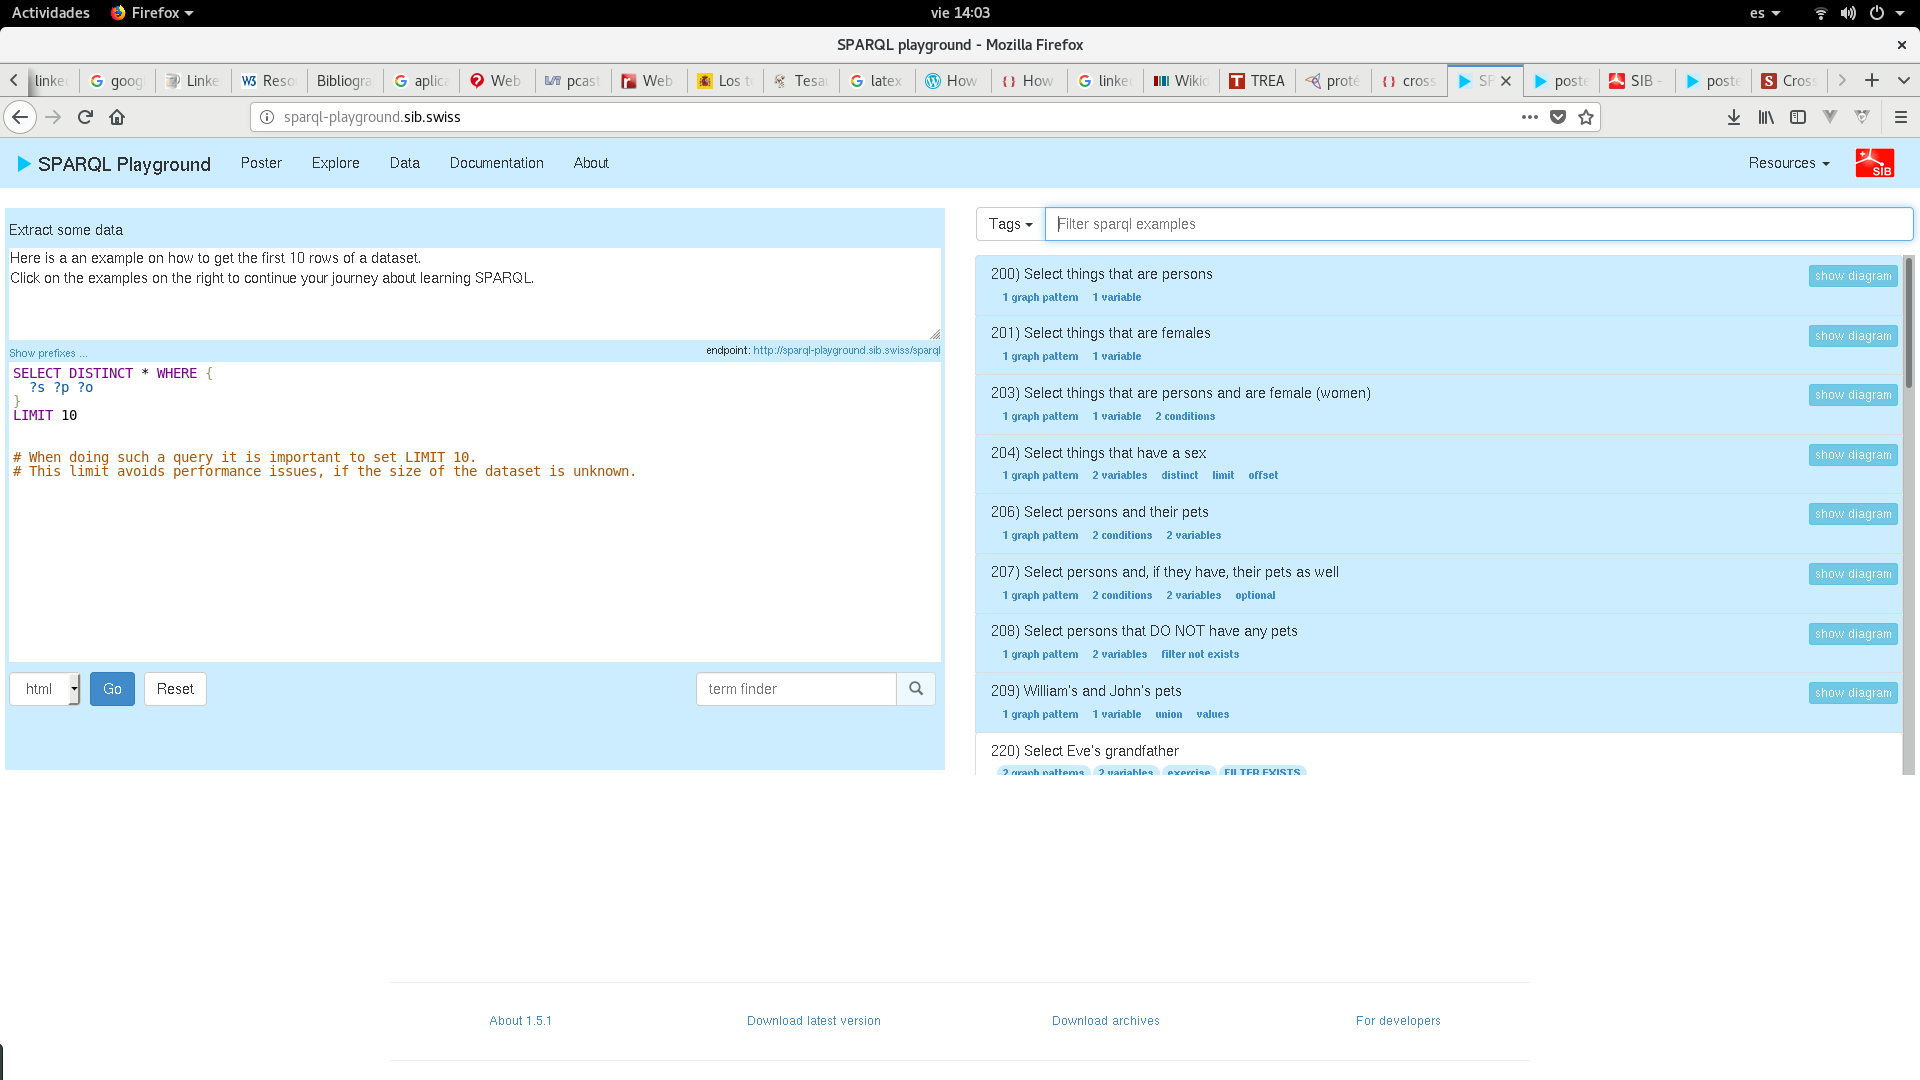
\includegraphics[scale=0.25]{sparql_playground}
	\caption{Interfaz de SPARQL \textit{playground}}
\end{figure}

Existan tambi�n bibliotecas de consulta para el \textit{frontend}, como Jassa (\textit{JAvascript Suite for Sparql Access})\footnote{http://aksw.org/Projects/Jassa.html}. Se trata de una biblioteca modular que comprende desde una API RDF sobre una capa de abstracci�n de servicios hasta una capa de navegaci�n por facetas. Sin embargo, desarrolla un modelo propio del grafo RDF no basado en est�ndares y se integra con versiones muy antiguas de Angular, lo que hace que pierda inter�s para su uso en producci�n.

\subsection{Herramientas de modelado}

\subsubsection{Herramientas web}

Existen pocas herramientas con funcionalidades de edici�n de grafos RDF en la Web. Al margen de la versi�n web de Prot�g�, cuya versi�n de escritorio (m�s representativa) se comenta en el punto \ref{deescritorio}, el resto de trabajos encontrados son fundamentalmente bibliotecas o paquetes de edici�n de formularios, como rdfforms\footnote{https://rdforms.org/}. Se trata de una biblioteca Javascript cuyo prop�sito es facilitar la construcci�n de editores RDF basados en formularios en un entorno web. Para ello, se basa en un mecanismo de plantillas que describe c�mo generar un formulario HTML y c�mo mapear expresiones espec�ficas en un grafo RDF a sus correspondientes campos.

Unas pruebas iniciales con la biblioteca sugirieron falta de madurez por fallos en su funcionamiento en un navegador. Adem�s, la biblioteca implementa su propio modelo de grafo RDF, que no est� relacionado con los est�ndares actuales (ver secci�n \ref{estadoactual}).

\begin{figure}[h]
	\centering
	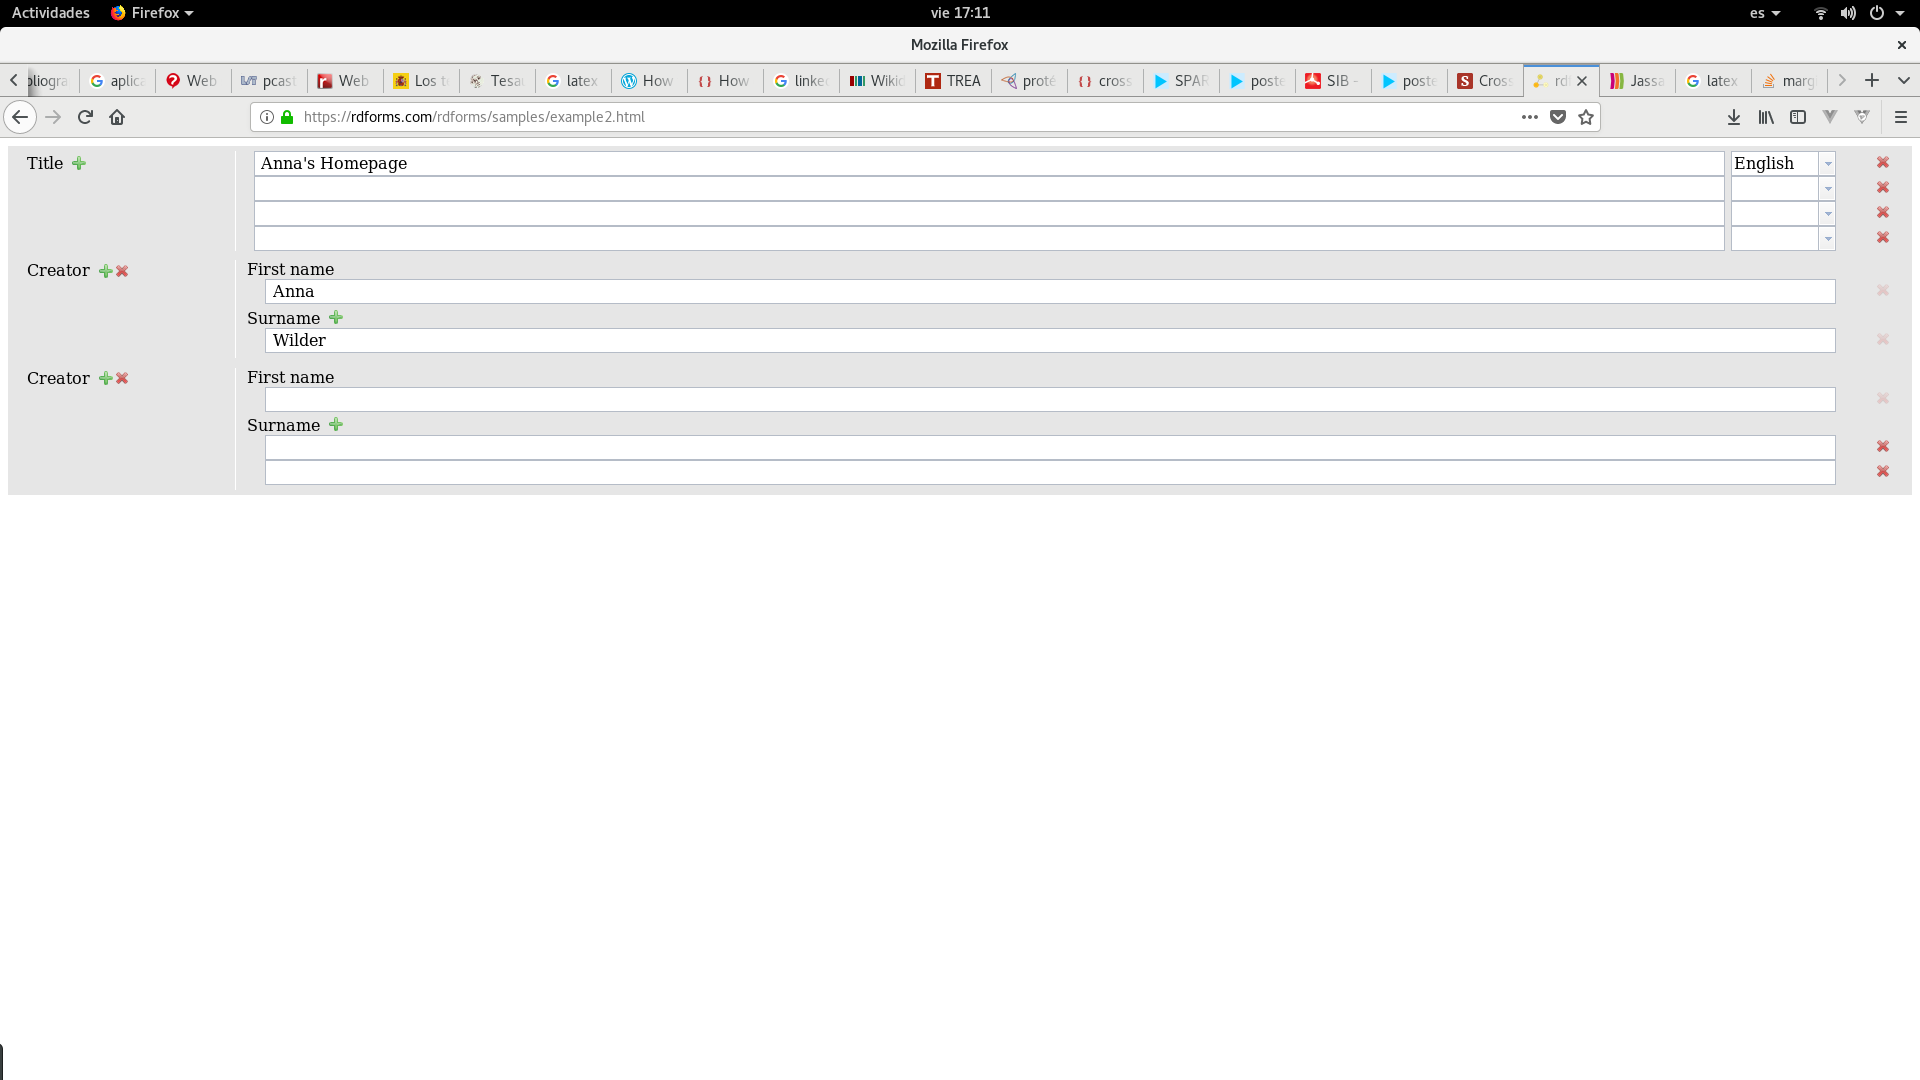
\includegraphics[scale=0.25]{rdfforms}
	\caption{Ejemplo de formulario desarrollado con rdfforms}
\end{figure}

\subsubsection{Herramientas de escritorio} \label{deescritorio}

La herramienta de modelado de ontolog�as en RDF por antonomasia es Prot�g�, un editor de ontolog�as \textit{opensource} gratuito y un marco de trabajo para construir sistemas inteligentes soportados por una fuerte comunidad de usuarios acad�micos, gubernamentales y corporativos. Se utiliza en �reas tan diversas como la biomedicina, el comercio electr�nico, la predicci�n metereol�gica o el modelado organizacional.

Prot�g� se instala como una aplicaci�n de escritorio multiplataforma y tiene una arquitectura basada en \textit{plugins} o complementos que permite extender f�cilmente su funcionalidad. Tiene soporte para razonadores sobre las distintas ontolog�as que se modelan y facilidades de representaci�n y edici�n de grafos RDF.

De cara a un primer encuentro con las tecnolog�as de la Web Sem�ntica, puede parecer abrumador por su gran flexibilidad y potencia. Adem�s, no cuenta con facilidades de consulta sobre los grafos modelados.

\begin{figure}[h]
	\centering
	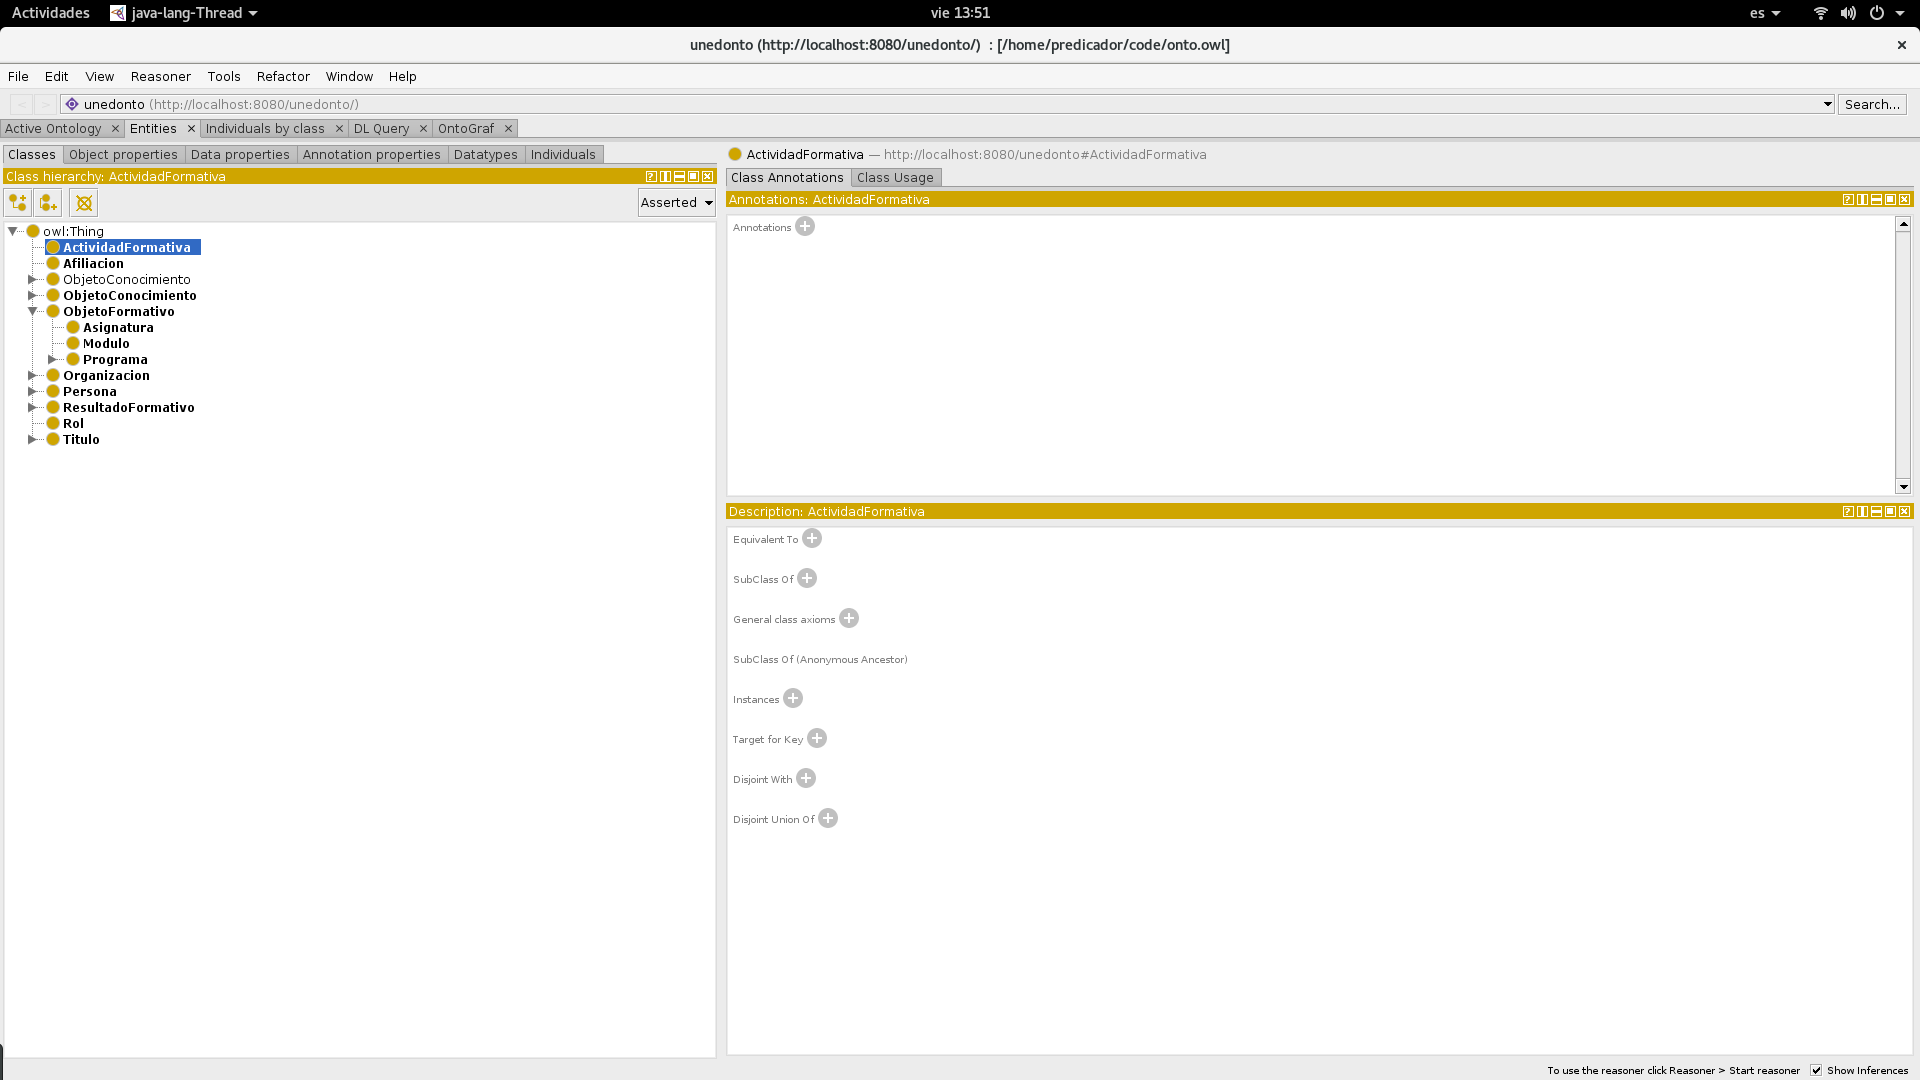
\includegraphics[scale=0.25]{protege}
	\caption{Interfaz de Prot�g�}
\end{figure}


\section{Estado actual} \label{estadoactual}

El estado actual (o \textit{state of the art}, del ingl�s) de las tecnolog�as de la Web Sem�ntica alcanza distintos niveles de madurez en sus implementaciones. Complementando el listado de herramientas ya presentado en el estudio de trabajos previos (\ref{trabajosprevios}), se analizan a continuaci�n las plataformas o bibliotecas m�s representativas dentro de las tecnolog�as m�s utilizadas.

\subsection{Java}

As�, para la plataforma Java se cuenta con Apache Jena{\cite{jena01}}, un marco de trabajo o \textit{framework} \textit{opensource} para construir aplicaciones para la Web Sem�ntica o sobre datos enlazados. De entre sus componentes y funcionalidades, cabe destacar:

\begin{itemize} 
\item \textbf{TDB}: una base de datos de tripletas nativa y de alto rendimiento, con excelente integraci�n con el resto de APIs de Jena.
\item \textbf{ARQ}: un motor SPARQL compatible con su versi�n 1.1 que soporta consultas federadas y b�squeda por texto libre.
\item \textbf{API RDF}: una API principal que permite interactuar con RDF para crear y leer grafos y tripletas, as� como serializarlas a los formatos m�s comunes (Turtle, XML, etc.).
\item \textbf{Fuseki}: un \textit{endpoint} SPARQL que permite exponer el grafo de trabajo y ofrece interacci�n tipo REST con tripletas RDF.
\item \textbf{Otras APIs}: como las de ontolog�as e inferencias, que permiten a�adir m�s sem�ntica al modelo y razonar sobre reglas por defecto o personalizadas.
\end{itemize}  

Apache Jena es una soluci�n robusta y muy utilizada en entornos acad�micos y de producci�n empresarial con m�s de quince a�os de vida.

\subsection{Python}

RDFLib\footnote{https://github.com/RDFLib/rdflib} es una biblioteca \textit{opensource} ligera pero funcionalmente completa para trabajar con RDF desde plataformas Python. Permite a las aplicaciones acceder a estructuras RDF a trav�s de construcciones idiom�ticas en Python, lo que facilita un acercamiento de la tecnolog�a al programador experimentado; por ejemplo, un grafo no es m�s que una colecci�n de tripletas \textit{<sujeto, predicado, objeto>}. Entre el resto de sus caracter�sticas, destacan:

\begin{itemize}
	\item Contiene procesadores y serializadores para XML, N3, Turtle, RDFa, etc.
	\item Presenta una interfaz para un grafo que puede soportarse sobre multitud de implementaciones de almacenes.
	\item Incluye una implementaci�n de SPARQL v1.1.
	\item Presenta una arquitectura modular basada en \textit{plugins} o complementos.
\end{itemize} 

Su desarrollo es estable y ha sido utilizada en referencias bibliogr�ficas como \textit{Programming the Semantic Web}\cite{evanstaylor01}, de\textit{ O'Reilly}.

\subsection{Javascript}

Dado que uno de los objetivos del proyecto es reducir al m�ximo los requisitos de uso de la herramienta para alcanzar el mayor p�blico objetivo posible (ver \ref{objetivos}), Javascript se presenta como una tecnolog�a de sumo inter�s, ya que permite producir aplicaciones ejecutables al cien por cien en un navegador web est�ndar.

Sin embargo, el \textbf{estado actual de implementaci�n de RDF en Javascript puede calificarse de inmaduro y e inestable}. Se han llevado a cabo intentos aislados de construir APIs RDF y herramientas para gesti�n de grafos y consultas SPARQL, como las citadas en la secci�n \ref{trabajosprevios}, pero no existe un est�ndar �nico consolidado (a�n).

En el W3C puede consultarse la mejor comparativa existente de bibliotecas desarrolladas en Javascript para trabajar con RDF\cite{rdfjscomparison}.

Sin duda, el esfuerzo m�s destacable hasta ahora para conseguir un est�ndar de RDF en Javascript es el proyecto rdflib.js\footnote{https://github.com/linkeddata/rdflib.js}, liderado por el mism�simo Tim Berners-Lee. Se trata de una biblioteca que proporciona una API local para lanzar consultas a un almac�n RDF, soporta parte de la especificaci�n SPARQL y permite importar y escribir formatos como RDF/XML, Turtle y N3. 

En el propio repositorio de rdflib.js se cita al \textit{ RDFJS Representation Task Force}\footnote{https://github.com/rdfjs/representation-task-force}, un grupo dentro del \textit{RDFJS Community Group}\footnote{https://www.w3.org/community/rdfjs/} encargado de dise�ar las especificaciones de interfaz con el objetivo de conseguir que las distintas implementaciones de conceptos RDF en Javascript sean interoperables. La especificaci�n de la interfaz existe en forma de borrador a fecha de 14 de Agosto de 2017\footnote{http://rdf.js.org/}. En ella se definen interfaces para t�rminos, cuaternas, factor�as de datos, nodos en blanco, literales, etc. as� como para \textit{streams} de Javascript.

Consultando el sitio web del \textit{Community Group} se puede encontrar una noticia del 23 de Abril de 2018 (publicada, por tanto, en pleno desarrollo de este proyecto) anunciando la creaci�n de RDF.js, que tratar� de unir los esfuerzos de distintas entidades (como la Universidad de Gante o el MIT) y alinear y publicar bajo un �nico paraguas proyectos como:

\pagebreak

\begin{itemize}
	\item El citado rdflib.js
	\item RDF-Ext, una biblioteca Javascript para trabajar con RDF y datos enlazados que cumple con la especificaci�n del RDFJS Representation Task Force.
	\item N3.js, una biblioteca que implementa la especificaci�n de bajo nivel RDF.js y permite leer, procesar, almacenar y exportar ternas RDF de forma as�ncrona en Javascript.
\end{itemize} 

Ante esta situaci�n confusa y repleta de distintas implementaciones, se opt� por utilizar canales de comunicaci�n directos con sus autores. Existen varios grupos de discusi�n en Gitter, tales como:

\begin{itemize}
	\item rdfjs/public\footnote{https://gitter.im/rdfjs/public}
	\item rdf-ext/discussions\footnote{https://gitter.im/rdf-ext/discussions}
\end{itemize} 

En ellos, el autor del proyecto tuvo la oportunidad de recibir indicaciones directamente de Thomas Bergwinkl, 


\section{Recursos}
\cleardoublepage{}

\chapter{Metodolog�a y Planificaci�n}

La metodolog�a y la planificaci�n son dos labores obligadas en cualquier proyecto de ingenier�a. No obstante, cabe aqu� citar la siguiente frase atribuida a Dwight D. Eissenhower: \blockquote[{\cite{eissenhower01}}]{Plans are worthless, but planning is everything.} Hay que tener en cuenta que una planificaci�n es tan s�lo una gu�a inicial para conseguir una organizaci�n m�s depurada durante el tiempo de desarrollo. La planificaci�n debe ser una herramienta flexible de ayuda, y no un instrumento r�gido que condicione otras caracter�sticas del sistema tales como su calidad. En las siguientes secciones se analizan con m�s detalle estos asuntos.

\section{Metodolog�a}

Para acometer este proyecto, se han valorado dos familias de metodolog�as de desarrollo de \textit{software}:

\begin{enumerate}
	\item Metodolog�as en cascada (\textit{Waterfall})
	\item Metodolog�as �giles (incrementales e iterativas)
\end{enumerate} 

La metodolog�a de desarrollo en cascada surgi� como idea en un art�culo de Winston W. Royce en 1970{\cite{royce01}}. Hist�ricamente, este modelo se ha extendido tanto en �mbitos acad�micos como profesionales, siendo estas sus principales caracter�sticas:

\begin{itemize}
	\item Gesti�n predictiva de proyectos llevada al software.
	\item Toma como modelo la forma de proceder en el resto de ingenier�as.
	\item Intenta llenar el vac�o del \textit{code \& fix}.
	\item Cada fase se realiza, en principio, una �nica vez.
	\item Cada fase produce un entregable que ser� entrada de la siguiente.
	\item Los entregables no son, en principio, modificables.
\end{itemize}

Es decir, se basa en la separaci�n entre dise�o y construcci�n (o entre creatividad y repetici�n).

La propuesta de Royce,tal y como se desprende de la lectura del art�culo original, describ�a el modelo en cascada como la \blockquote[{\cite{royce01}}]{descripci�n m�s simple} que solo funcionar�a para los proyectos m�s sencillos. Ir�nicamente, este mensaje malentendido ha sido el origen de la popularidad de la metodolog�a en cascada, que hoy en d�a se sigue promoviendo en muchos casos por inercia, desconocimiento, comodidad o ilusi�n de control sobre el proyecto.
 
Lamentablemente, en la \textit{Ingenier�a de Software} los pesos de dise�o y construcci�n est�n invertidos con respecto a otras ingenier�as, siendo el \textit{software} un dominio de cambio y alta inestabilidad. El desarrollo de \textit{software} es, intr�nsecamente, una labor creativa; y la creatividad no es f�cilmente predecible. Esto ha dado lugar a que los desarrollos tradicionales adolezcan de ciertos problemas{\cite{larman01}}:

\begin{itemize}
	\item Existencia de muchos requisitos vagos o especulativos y dise�o detallado por adelantado.
	\item Est�n fuertemente asociados con las tasas de fallo m�s altas en proyectos.
	\item Se encuentran promovidos hist�ricamente por creencia m�s que por evidencia estad�stica significativa.
	\item Su rigidez incrementa el riesgo de fracaso, pospuesto hasta las fases finales del proyecto.
	\item Asume que las especificaciones son predecibles, estables y completas.
	\item Pospone integraci�n y pruebas hasta fases tard�as.
	\item Se basa en estimaciones y planificaci�n ``fiables''.
\end{itemize}

Entre los estudios que ratifican las afirmaciones anteriores, cabe citar los siguientes:

\begin{itemize}
	\item Informe Chaos 2015\cite{chaos15}.
	\item \textit{Dr. Dobb's Journal article The Non'Existent Software Crisis: Debunking the Chaos Report}\cite{ambler01}.
	\item Encuesta de Gartner\cite{mieritz01}.
    \item TODO
\end{itemize}

Por tanto, atendiendo a esta exposici�n y considerando que el proyecto en cuesti�n presentaba un alto nivel de incertidumbre debido a su alto componente en investigaci�n del estado tecnol�gico actual, se ha optado por utilizar un enfoque metodol�gico incremental e iterativo, puesto que:

\begin{itemize}
	\item Facilita llevar a cabo proyectos peque�os.
	\item Fomenta la interacci�n entre el desarrollador y el usuario.
	\item Fuerza a que los inevitables cambios en requisitos sucedan en fases tempranas del proyecto.
\end{itemize}

Entre sus caracter�sticas es posible citar:

\begin{itemize}
	\item Se trabaja sobre subconjuntos de funcionalidad (\textit{features}).
	\item Los incrementos permiten a�adir funcionalidad al producto (mejora del proceso).
	\item Las iteraciones permiten redise�ar, revisar y refactorizar el producto (mejora del producto).
	\item Se basa en entregas frecuentes y ciclos prueba/error.
	\item Ofrece flexibilidad a la hora de gestionar el cambio.
\end{itemize}

La referencia m�s clara en este �mbito es \textit{Extreme Programming}, de Kent Beck\cite{beck01}. \textit{Extreme Programming} es \blockquote[{\cite{royce01}}]{un estilo de desarrollo de software centrado en la aplicaci�n excelente de t�cnicas de programaci�n, comunicaci�n clara y trabajo en equipo que permite conseguir objetivos antes impensables}. Se trata de una metodolog�a basada en valores como la comunicaci�n, realimentaci�n, simplicidad, valent�a y respeto, soportada sobre un cuerpo de pr�cticas �tiles y con un conjunto de principios complementarios, adem�s de contar con una comunidad de usuarios que comparte todo lo anterior.

Su aplicaci�n al desarrollo de este proyecto no ha sido estricta; por ejemplo, no se han definido ciclos estrictos por la propia naturaleza inestable de la dedicaci�n al desarrollo del mismo, pero s� que ha realizado un dise�o evolutivo soportado sobre un n�mero suficiente de pruebas unitarias as� como una planificaci�n incremental y adaptativa a las problem�ticas que iban surgiendo.

Prueba del acierto a la hora de elegir esta metodolog�a es el cambio de necesidades y requisitos funcionales que tuvo lugar en la reuni�n presencial mantenida con el tutor, donde \textbf{la metodolog�a aport� que no fuera necesario descartar ning�n desarrollo o trabajo realizado hasta la fecha}. Permiti� realizar una gesti�n del cambio efectiva, re-orientando el trabajo a tiempo sin impactar en el dise�o ni en la implementaci�n existente. Finalmente, tanto la organizaci�n como la planificaci�n de las tareas han sido lo suficientemente flexibles para conseguir un ritmo adecuado de desarrollo, reduciendo los puntos de bloqueo.

\section{Planificaci�n}


\subsection{Planificaci�n global}

Para realizar la planificaci�n del proyecto, y dada la metodolog�a de desarrollo incremental e iterativa elegida, no se ha seguido un modelo t�pico en fases de \textit{An�lisis, Dise�o, Implementaci�n, etc.} sino que se ha optado por un enfoque orientado a tareas relacionadas con la funcionalidad del producto final esperado.

\begin{figure}[h]
	\begin{ganttchart}[
		canvas/.append style={fill=none, draw=black!5, line width=.75pt},
		hgrid style/.style={draw=black!5, line width=.75pt},
		vgrid={*1{draw=black!5, line width=.75pt}},
		title/.style={draw=none, fill=none},
		title label font=\bfseries\footnotesize,
		title label node/.append style={below=4pt},
		include title in canvas=false,
		bar label font=\mdseries\small\color{black!70},
		bar label node/.append style={left=2cm},
		bar/.append style={draw=none, fill=black!63},
		bar incomplete/.append style={fill=barblue},
		bar progress label font=\mdseries\footnotesize\color{black!70},
		group/.append style={draw=none, fill=groupblue},
		group left shift=0,
		group right shift=0,
		group height=.5,
		group peaks tip position=0,
		group label node/.append style={left=.6cm},
		group progress label font=\bfseries\small,
		link/.style={-latex, line width=1.5pt, linkred},
		link label font=\scriptsize\bfseries,
		link label node/.append style={below left=-2pt and 0pt}
		]{1}{20}
		\gantttitle{Planificaci�n inicial}{20} \\
		\gantttitle{Febrero}{4}
		\gantttitle{Marzo}{4}
		\gantttitle{Abril}{4}
		\gantttitle{Mayo}{4}
		\gantttitle{Junio}{4}\\
		\gantttitle[
		title label node/.append style={below left=4pt and -3pt}
		]{Semana:\quad1}{1}
		\gantttitlelist{2,...,20}{1} \\
		\ganttgroup[]{Documentaci�n y arranque}{1}{4} \\
		\ganttgroup[]{Prueba de concepto}{4}{8} \\
		\ganttgroup[]{Desarrollo del proyecto}{8}{14} \\
		\ganttgroup[]{Resultados y memoria}{14}{20} \\
	\end{ganttchart}
	\caption{Planificaci�n inicial}\label{fig:gantt01}
\end{figure}

\pagebreak

La figura anterior (\ref{fig:gantt01}) muestra la planificaci�n propuesta para la elaboraci�n del anteproyecto.

En esta propuesta era clave la revisi�n de la prueba de concepto con el tutor para comprobar que efectivamente se hab�an comprendido las necesidades desprendidas del an�lisis y para poder continuar con la especificaci�n funcional de forma m�s refinada y precisa.

En la pr�ctica, la evoluci�n del proyecto ha sido bien distinta. En la figura \ref{fig:gantt02} se puede comprobar cu�l ha sido la planificaci�n efectiva, producto esta de cambios sobre la inicial para resolver los distintos imprevistos que han ido surgiendo durante la ejecuci�n del mismo.

\begin{figure}
	\begin{changemargin}{-1cm}{-1cm}
		\begin{tikzpicture}[y=0.50cm] 
		\begin{ganttchart}[
		y unit chart=0.8cm,
		canvas/.append style={fill=none, draw=black!5, line width=.75pt},
		hgrid style/.style={draw=black!5, line width=.75pt},
		vgrid={*1{draw=black!5, line width=.75pt}},
		title/.style={draw=none, fill=none},
		title label font=\bfseries\footnotesize,
		title label node/.append style={below=4pt},
		include title in canvas=false,
		bar label font=\mdseries\tiny\color{black!70},
		bar label node/.append style={left=0.5cm},
		bar/.append style={draw=none, fill=barblue!63},
		bar incomplete/.append style={fill=barblue},
		bar progress label font=\mdseries\footnotesize\color{black!70},
		group incomplete/.append style={fill=groupblue},
		group/.append style={draw=none, fill=groupblue},
		group left shift=0,
		group right shift=0,
		group height=.5,
		group peaks tip position=0,
		group label node/.append style={left=.6cm},
		group label font=\bfseries\tiny,
		milestone label font=\bfseries\tiny,
		link/.style={-latex, line width=1.5pt, linkred},
		link label font=\scriptsize\bfseries,
		link label node/.append style={below left=-2pt and -5pt}
		]{1}{28}
		\gantttitle{Planificaci�n efectiva}{28} \\
		\gantttitle{Febrero}{2}
		\gantttitle{Marzo}{4}
		\gantttitle{Abril}{4}
		\gantttitle{Mayo}{4}
		\gantttitle{Junio}{4}
		\gantttitle{Julio}{4}
		\gantttitle{Agosto}{4}
		\gantttitle{Septiembre}{2}\\
		\gantttitle[
		title label node/.append style={below left=4pt and -6pt}
		]{Semana:\quad1}{1}
		\gantttitlelist{2,...,28}{1} \\
		\ganttgroup[]{Formaci�n y arranque (FA)}{1}{6} \\
		\ganttbar[
		name=FA11
		]{\textbf{FA 1.1} RDF y OWL}{1}{2} \\
		\ganttbar[
		name=FA12
		]{\textbf{FA 1.2} JS ES6+, Vue}{3}{6} \\
		\ganttbar[
		name=FA13
		]{\textbf{FA 1.3} POC edici�n tripleta}{1}{6} \\
		\ganttmilestone{Prueba de concepto inicial}{6}{6} \\
		\ganttbar[
		name=FA14
		]{\textbf{FA 1.4} An�lisis de necesidades}{1}{6} \\
		\ganttgroup[]{Desarrollo de m�dulo de edici�n (ME)}{7}{20} \\
		\ganttbar[]{\textbf{ME 2.1} Plantilla Vue + testing}{7}{8} \\
		\ganttbar[]{\textbf{ME 2.2} Dise�o de componentes}{8}{9} \\
		\ganttbar[]{\textbf{ME 2.3} Implementaci�n CRUD clases}{9}{13} \\
		\ganttbar[]{\textbf{ME 2.4} Implementaci�n export/import}{12}{14} \\
		\ganttbar[]{\textbf{ME 2.5} Mejoras en visualizaci�n y uso }{14}{16} \\
		\ganttbar[]{\textbf{ME 2.6} Refactorizaci�n y generalizaci�n }{16}{20} \\
		\ganttbar[]{\textbf{ME 2.7} Pruebas}{7}{20} \\
		\ganttmilestone{Reuni�n presencial}{20}{20} \\
		\ganttgroup[]{Desarrollo de m�dulos playground}{20}{25} \\
		\ganttbar[]{\textbf{ME 3.1} M�dulo de consulta SPARQL}{20}{23} \\
		\ganttbar[]{\textbf{ME 3.2} M�dulo de carga de actividades}{23}{24} \\
		\ganttbar[]{\textbf{ME 3.3} M�dulo de carga de vocabularios}{23}{24} \\
		\ganttbar[]{\textbf{ME 3.4} Mejoras en la importaci�n}{23}{24} \\
		\ganttbar[]{\textbf{ME 3.5} Revisi�n, refactoring, cleaning}{24}{25} \\
		\ganttbar[]{\textbf{ME 3.6} Pruebas}{20}{25} \\
		\ganttgroup[]{Redacci�n de memoria y cierre}{24}{28} \\
		\ganttbar[]{\textbf{ME 4.1} Formaci�n latex}{24}{24} \\
		\ganttbar[]{\textbf{ME 4.2} Redacci�n memoria}{24}{28} \\
		
		\end{ganttchart}
		\end{tikzpicture}
	\end{changemargin}
	\caption{Planificaci�n efectiva}\label{fig:gantt02}
\end{figure}

Con respecto a la planificaci�n inicial, se tiene que:

\begin{itemize}
	\item El proyecto se ha retrasado un total de ocho semanas.
	\item El per�odo de formaci�n llev� al menos dos semanas m�s de lo esperado (en realidad, el aprendizaje del \textit{framework Vue} ha estado presente a lo largo de pr�cticamente todo el desarrollo del proyecto).
	\item El desarrollo del producto ha consumido seis semanas m�s de las previstas inicialmente.
	\item La memoria se ha redactado en dos semanas menos con respecto a la estimaci�n inicial.
\end{itemize} 

Las desviaciones surgidas con respecto a la planificaci�n inicial tienen su explicaci�n en los siguientes motivos:

\begin{itemize}
	\item El alto grado de incertidumbre a la hora de estimar la planificaci�n inicial, dado que se desconoc�a cu�l era la situaci�n actual del ecosistema tecnol�gico de \textit{front-end web} y su integraci�n con las tecnolog�as de la Web Sem�ntica.
	\item La curva de aprendizaje de \textit{Vue}, si bien es considerada m�s suave que la de sus competidores (\textit{React, Angular}) fue mayor de lo esperado. El bajo grado de familiarizaci�n del autor del proyecto con las tecnolog�as de \textit{front-end} y, especialmente, \textit{Javascript ES6+}, no facilit� el aprendizaje.
	\item El\textbf{ bajo nivel de madurez de las bibliotecas existentes} para la manipulaci�n de RDF en Javascript, as� como la heterogeneidad y poca estabilidad de estas implementaciones, ha suscitado muchas dudas sobre cu�les utilizar y c�mo enfocar su integraci�n con \textit{frameworks} m�s maduros como \textit{Vue}.
	\item La \textbf{pr�ctica ausencia de bibliotecas} o componentes de interacci�n con SPARQL \textbf{conformes a la especificaci�n est�ndar de la interfaz} \textit{rdf.js}{\cite{rdfjs01}} (que por otra parte, es un borrador de 2017) ha puesto en peligro la viabilidad del proyecto. La plataforma finalmente utilizada, \textit{Comunica}{\cite{comunica01}}, a�n no tiene una versi�n estable muchos de sus m�dulos (concretamente, el endpoint SPARQL utilizado para el proyecto no la tiene), con lo que ha sido necesario estar en contacto directo con sus autores y colaborar con ellos en la revisi�n de defectos o \textit{bugs} y dependiendo por tanto de sus tiempos de respuesta (hay que tener en cuenta que la plataforma es \textit{opensource} y por tanto no existe acuerdo de nivel de servicio alguno.)
	\item La dificultad existente en llevar a cabo un an�lisis de requisitos a trav�s de una plataforma online de colaboraci�n como puede ser \textit{Skype}: para constatar este hecho no hay m�s que verificar el cambio de rumbo del proyecto una vez mantenida la reuni�n presencial, que sirvi� para definir objetivos m�s claros y comprender las necesidades del Departamento.
\end{itemize} 

A pesar de todo ello, el autor de este proyecto est� satisfecho con el nivel de conocimiento adquirido en el �mbito de todas las tecnolog�as empleadas y el tiempo consumido para obtener como resultado un producto desplegado en producci�n y listo para utilizar.


\subsection{Planificaci�n �gil} \label{subsec:agileplanning}

Si bien para la planificaci�n global del proyecto se han utilizado herramientas tales como el \textit{diagrama de Gantt}, para gestionar el trabajo del d�a a d�a otro enfoque ha sido necesario. En el contexto de metodolog�as �giles de desarrollo de software de tipo incremental e iterativo como Extreme Programming, \textbf{las tareas de planificaci�n adquieren un car�cter adaptativo} muy distinto del que presenta una planificaci�n tradicional con una metodolog�a de desarrollo en cascada, por ejemplo.

La planificaci�n �gil es un proceso en continua evoluci�n, tambi�n iterativo e incremental como las metodolog�as a las que pertenece, basada en ciclos del tipo:

\begin{enumerate}
	\item A�adir tareas
	\item Estimar tareas
	\item Priorizar tareas
\end{enumerate}

En este caso, la estimaci�n de tareas se llev� a cabo de forma heur�stica, utilizando la experiencia del autor y el conocimiento del contexto existente en el momento de la estimaci�n. En base a ello, la priorizaci�n (ordenaci�n) de las tareas ten�a lugar inmediatamente, relegando a la estimaci�n a un segundo plano.

Para gestionar estas tareas, se ha optado por utilizar como herramienta Kanban. Un tablero Kanban puede definirse como un dispositivo de se�alizaci�n que introduce el flujo de trabajo de un proceso a un ritmo manejable. Presenta las siguientes caracter�sticas:


\begin{itemize}
	\item Solo env�a trabajo cuando lo ordena el cliente o usuario (en este caso, el propio autor del proyecto)
	\item Indica espec�ficamente qu� trabajo debe hacerse.
	\item Controla la cantidad de trabajo en progreso.
	\item Regula las interrupciones y orquesta el ritmo de trabajo.
\end{itemize} 


B�sicamente, consiste en utilizar una tabla con varias columnas para visualizar el estado de una tarea a lo largo de las distintas fases que se consideren. Para el caso de la realizaci�n de este proyecto, se crearon las siguientes columnas:

\begin{center}
	\begin{table}[htb]
		\centering
		\begin{tabular}{p{3cm}p{10cm}}
			\toprule
			Columna & Descripci�n \\
			\toprule
			To-Do & Tareas por realizar en orden de prioridad descendente \\ \midrule
			Work in progress & Tareas realiz�ndose en un momento dado. No m�s de dos o tres. \\ \midrule
			Stand-by & Tareas a la espera por motivos ajenos al autor del proyecto. \\ \midrule
			Done & Tareas finalizadas. \\ \midrule
			Discarded & Tareas descartadas debido a cambios de dise�o, requisitos, etc. \\ \midrule
			Doubts & Dudas planteadas a lo largo del desarrollo del proyecto. \\ \midrule
			Resources & Recursos documentales en la web �tiles para del desarrollo del proyecto. \\
			\bottomrule
		\end{tabular}
		\caption{Dise�o del tablero Kanban}
		\label{tabkanban}
	\end{table}
\end{center}

\begin{figure}[h]
	\centering
	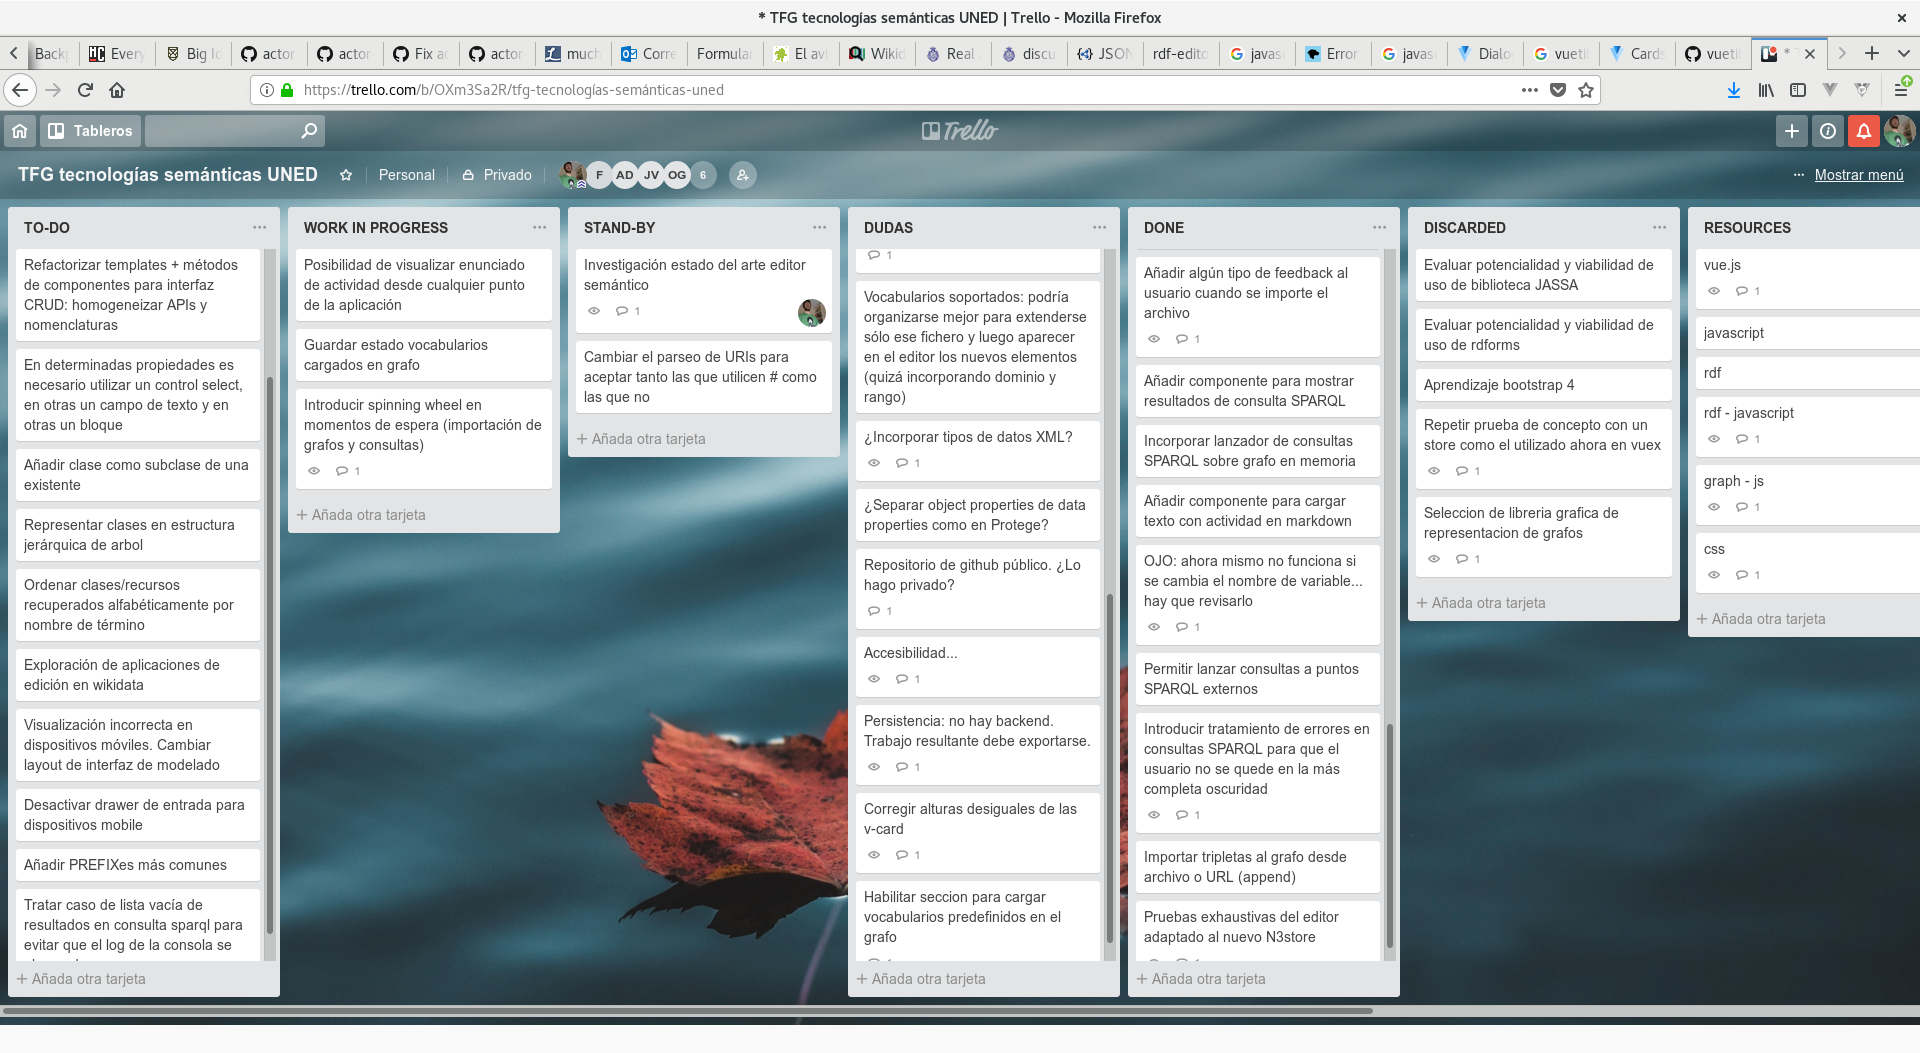
\includegraphics[scale=0.25]{trello}
	\caption{Ejemplo de tablero Trello}
\end{figure}


\cleardoublepage{}

\chapter{An�lisis}

\section{Captura y documentaci�n de requisitos}

\subsection{Captura de requisitos}

La t�cnica de captura de requisitos utilizada para este proyecto ha sido, fundamentalmente, \textbf{la entrevista} con el tutor. Se eligi� esta t�cnica por los siguientes motivos:

\begin{itemize}  
	\item Las entrevistas, bien a distancia o presenciales (y especialmente estas �ltimas), permiten una mayor implicaci�n del usuario en la captura de requisitos.
	\item Combinada con una maqueta o prueba de concepto, una entrevista presencial puede dar lugar a la aparici�n de nuevos requisitos de producto, cambios en las especificaciones e incluso en el enfoque y objetivos del mismo.
	\item Permite la pr�ctica de la escucha activa y la sugerencia de ideas por parte del analista, aportando un valor a�adido que enriquece la simple captura de requisitos.
	\item Es claramente la t�cnica m�s obvia, directa y accesible en el contexto de la realizaci�n del proyecto.
\end{itemize}

Concretamente, se han llevado a cabo varias entrevistas utilizando la plataforma colaborativa Skype y una presencial, en la que el autor de este proyecto se ha desplazado a la sede del departamento en Madrid con objeto de conseguir una comunicaci�n m�s fluida y un mayor entendimiento a la hora de consensuar las necesidades y funcionalidades requeridas del producto.

La primera entrevista a distancia propici� un intercambio de documentos e ideas que desemboc� en la elaboraci�n del documento del anteproyecto. El resto de entrevistas a trav�s de Skype sirvieron para concretar en mayor medida las tareas a realizar y el enfoque del proyecto. Sin embargo, no fue hasta que no tuvo lugar la reuni�n presencial cuando realmente se le dio al proyecto su orientaci�n final, con unos objetivos claramente definidos y una posibilidad para cumplir los hitos propuestos.

A continuaci�n se resumen todas las sesiones de captura de requisitos:

\vspace*{\baselineskip}
\begin{center}
\begin{table}[htb]
\centering
\begin{tabular}{p{1cm}p{2cm}p{10cm}}
	\toprule
	id & Fecha & Resumen de la entrevista \\
	\toprule
	1 & 18/10/17 & Primer contacto y comunicaci�n de ideas iniciales para la confecci�n del anteproyecto  \\ \midrule
	2 & 21/02/17 & Consolidaci�n de ideas y aportaci�n de m�s documentaci�n (v�deos sobre prototipos de cuaderno, documentos de texto con descripciones, etc.)  \\
	3 & 28/03/18 & Primera demo a modo de POC con un entorno capaz de a�adir tripletas.  \\ \midrule
	4 & 10/07/18 & Reuni�n presencial con demostraci�n \textit{in-situ} de los m�dulos de modelado e importaci�n/exportaci�n. Tiene lugar una tormenta de ideas y se enfoca el proyecto de otro modo, modificando sus objetivos hacia una herramienta formativa..  \\ \midrule
	5 & 4/08/18 & Revisi�n de los �ltimos avances con la integraci�n de un endpoint SPARQL en el frontend y planificaci�n del resto de funcionalidade requeridas.  \\ 
	\bottomrule
\end{tabular}
\caption{Sesiones de entrevistas}
\label{tabmeetings}
\end{table}
\end{center}

\subsection{Documentaci�n}

Para documentar la captura de requisitos, se utilizar� la t�cnica de casos de uso. Se descarta la incorporaci�n de diagramas UML de casos de uso, dado que dichos diagramas carecen de informaci�n esencial sobre los mismos (como qu� actor lleva a cabo cada paso, o notas sobre el orden de ejecuci�n de los pasos). Si bien pueden ser �tiles como resumen o �ndice de contenidos, se decide prescindir de ellos dado que el n�mero de casos de uso contemplados en el proyecto es manejable.

Se utilizar� una plantilla propuesta por Cockburn{\cite{cockburn01}}: el estilo RUP (\textit{Rational Unified Process}){\cite{rational01}}, atractivo y f�cil de seguir pese al elevado n�mero de apartados, modificado para plasmar los aspectos m�s relevantes del proyecto (por ejemplo, no se incluir� un campo \textit{�mbito} porque siempre va a estar referido al mismo sistema o aplicaci�n). El motivo de no utilizar una tabla es meramente subjetivo, ya que el autor de esta memoria opina que puede oscurecer el contenido.

La plantilla sigue la siguiente estructura:

\begin{enumerate}  
	\item Nombre del caso de uso
	\begin{enumerate}
		\item Descripci�n breve
		\item Actores, entre los que estar� el actor principal. Presentan comportamiento.
		\item Disparadores: acciones sobre el sistema que inician los casos de uso.
	\end{enumerate}
	\item Flujo de eventos
		\begin{enumerate}
		\item Flujo b�sico: escenario principal de �xito.
		\item Flujos alternativos: qu� puede pasar que no sea el flujo principal.
			\begin{enumerate}
			\item Condicion 1
			\item Condici�n 2
			\item \ldots
		\end{enumerate}
	\end{enumerate}
	\item Requisitos especiales (si se dieran): plataforma, etc.
	\item Precondiciones: qu� debe ser cierto antes de ejecutar el caso de uso.
	\item Postcondiciones: qu� debe ser cierto despu�s de ejecutar el caso de uso.
\end{enumerate}

Los requisitos fueron capturados inicialmente como notas manuscritas y convertidos en necesidades de alto nivel en la plataforma Trello. A partir de ah�, dichas necesidades se refinaron para dar lugar a la bater�a de casos de uso incluida en \ref{sec:53}.

\section{Necesidades}

La reuni�n presencial marc� un punto de inflexi�n en cuanto a objetivos del proyecto, lo que se traduce en un cambio de necesidades. Para reflejar la evoluci�n completa, se dividir� su captura en dos fases detalladas a continuaci�n:

\subsection{Captura inicial}

A continuaci�n se resumen, en lenguaje natural, las necesidades identificadas durante la primera fase de desarrollo del proyecto:
\begin{enumerate}
\item Permitir a usuarios de la UNED  de distintos colectivos etiquetar y generar sus propios cuadernos con informaci�n y metainformaci�n sem�ntica.
\item Permitir a dichos usuarios realizar consultas sobre sus cuadernos.
\item Desarrollar una interfaz web que permita al usuario gestionar tripletas RDF.
\item Desarrollar un m�dulo de generaci�n de consultas SPARQL a partir de consultas de lectura y escritura en formato JSON.
\item Desarrollar los correspondientes productos de inter�s para el usuario: consultas exportadas en forma diversa (CSV, JSON) o embebidas en una plantilla HTML significativa para el usuario.
\item Ofrecer la posibilidad de variar interfaces de entrada y exportadores en funci�n de los distintos colectivos de usuario utilizando los metadatos sobre cuadernos RDF previamente almacenados en una base de datos relacional.
\item Permitir mostrar en pantalla una serie de t�rminos como punto de partida que el usuario pueda utilizar para construir ternas RDF y relaciones entre ellas.
\item Permitir mostrar en pantalla una serie de t�rminos como punto de partida que el usuario pueda utilizar para construir ternas RDF y relaciones entre ellas.
\item Ofrecer al usuario una visualizaci�n sencilla y correcta de su modelo que proporciona una perspectiva adecuada sobre la que trabajar.
\item Presentar una interfaz de mantenimiento del grafo: vocabulario e instancias (conceptualizaci�n y poblamiento de una ontolog�a).
\item Importar y exportar informaci�n estructurada en formatos sem�nticos est�ndar.
\item Extender con vocabularios tales como SKOS y OWL. 
\end{enumerate}

\subsection{Captura final}

Una vez celebrada la reuni�n presencial, se decidi� darle otro enfoque al proyecto. Si bien la idea inicial era desarrollar un sistema que permitiese generar cuadernos a trav�s de la manipulaci�n de grafos, una vez presentada una maqueta o prueba de concepto con funcionalidades b�sicas de modelado el tutor propuso convertir la herramienta en un \textit{playground} o sistema de realizaci�n de actividades acad�micas con un enfoque docente orientado a facilitar el aprendizaje de las tecnolog�as de la Web Sem�ntica (b�sicamente RDF y SPARQL) a personas con poco o ning�n contacto con estas materias (por ejemplo, alumnos de los Grados de Ingenier�a Inform�tica o en Tecnolog�as de la Informaci�n de la UNED).

Este nuevo enfoque se tradujo en la siguiente instant�nea de necesidades de alto nivel:

\begin{enumerate}
\item Permitir el modelado sem�ntico con edici�n CRUD de clases, subclases y propiedades de clases (anotaciones b�sicas).
\item Permitir la edici�n CRUD de relaciones o propiedades, subpropiedades, etc.
\item Ofrecer mecanismos de poblamiento del grafo.
\item Permitir el lanzamiento de consultas SPARQL sobre el grafo local y visualizaci�n de resultados.
\item Permitir el lanzamiento de consultas SPARQL sobre endpoints remotos y visualizaci�n de resultados.
\item Ofrecer funcionalidad de carga de consultas SPARQL predefinidas desde archivo de texto.
\item Incorporar m�dulo para a�adir un texto con la definici�n de la actividad a realizar en formato Markdown.
\item Permitir la importaci�n de tripletas desde archivos o URL.
\item Permitir la incorporaci�n (append) de tripletas al grafo local desde archivos o URL.
\item Ofrecer un panel para cargar en el grafo vocabularios comunes predefinidos.
\item Presentar una interfaz f�cil de usar y responsiva para el usuario, con una gesti�n de errores adecuada y suficiente.
\end{enumerate}

\section{Casos de uso} \label{sec:53}

\subsection{Dar de alta una nueva clase}

\subsubsection{Descripci�n breve}

Este caso de uso permite a un usuario a�adir una nueva clase a su grafo a trav�s de una tripleta que tendr� como sujeto el nombre de la clase, como objeto el recurso owl:Class y como predicado el recurso rdf:type. 

\subsubsection{Actores}

El actor principal es el usuario de la aplicaci�n (fundamentalmente dirigida a un alumno, pero podr�a ser un profesor o cualquier otro usuario).

\subsubsection{Disparadores}

El caso de usa comienza cuando el usuario pulsa en el bot�n flotante + asociado a la tarjeta del listado de clases.

\subsubsection{Flujo de eventos}
\begin{enumerate}
	\item Flujo b�sico
	\begin{enumerate}
		\item El usuario pulsa en el bot�n flotante + asociado a la tarjeta del listado de clases.
		\item Aparece un cuadro de di�logo donde el usuario debe introducir el nombre de la clase.
		\item El usuario introduce el URI del recurso que quiere dar de alta como clase y pulsa en guardar.
		\item El nuevo recurso de tipo clase se crea y aparece en el listado de clases.
	\end{enumerate}
	\item Flujo alternativo 1
\begin{enumerate}
	\item El usuario pulsa en el bot�n flotante + asociado a la tarjeta del listado de clases.
	\item Aparece un cuadro de di�logo donde el usuario debe introducir el nombre de la clase.
	\item El usuario introduce (o no) el URI del recurso que quiere dar de alta como clase y pulsa fuera del cuadro de di�logo.
	\item El cuadro de di�logo se cierra y no hay ning�n cambio en los recursos.
\end{enumerate}
	\item Flujo alternativo 2
	\begin{enumerate}
		\item El usuario pulsa en el bot�n flotante + asociado a la tarjeta del listado de clases.
		\item Aparece un cuadro de di�logo donde el usuario debe introducir el nombre de la clase.
		\item El usuario introduce el URI del recurso que quiere dar de alta como clase y pulsa en guardar.
		\item Ocurre un error en el guardado del recurso que le es comunicado al usuario a trav�s de una notificaci�n en pantalla.
	\end{enumerate}

\end{enumerate}

\subsubsection{Requisitos especiales}

Ninguno.

\subsubsection{Precondiciones}

El usuario debe haber navegado previamente hasta la secci�n de modelado, bien a trav�s de la pantalla de bienvenida, bien a trav�s de la barra de navegaci�n lateral.

\subsubsection{Postcondiciones}

Ninguna.

\subsubsection{Extensiones}

Ninguna.

\subsection{Editar una clase existente}

\subsubsection{Descripci�n breve}

Este caso de uso permite a un usuario editar el recurso asociado a una clase existente en su grafo y cambiar su URI.

\subsubsection{Actores}

El actor principal es el usuario de la aplicaci�n (fundamentalmente dirigida a un alumno, pero podr�a ser un profesor o cualquier otro usuario).

\subsubsection{Disparadores}

El caso de usa comienza cuando el usuario pulsa en el icono de men� asociado a la clase que quiere editar y selecciona la acci�n ``Editar''.

\subsubsection{Flujo de eventos}
\begin{enumerate}
	\item Flujo b�sico
	\begin{enumerate}
		\item El usuario pulsa en el icono de men� asociado a la clase que quiere editar y selecciona la acci�n ``Editar''.
		\item Aparece un cuadro de di�logo con el URI del recurso actual que el usuario puede modificar.
		\item El usuario modifica (o no) el URI del recurso  y pulsa en guardar.
		\item El recurso ha sido modificado y su cambio se ve reflejado en el listado.
	\end{enumerate}
\item Flujo alternativo 1
\begin{enumerate}
	\item El usuario pulsa en el icono de men� asociado a la clase que quiere editar y selecciona la acci�n ``Editar''.
	\item Aparece un cuadro de di�logo con el URI del recurso actual que el usuario puede modificar.
	\item El usuario modifica (o no) el URI del recurso  y pulsa fuera del cuadro de di�logo.
	\item El cuadro de di�logo se cierra y no hay ning�n cambio en los recursos.
\end{enumerate}
	\item Flujo alternativo 2
	\begin{enumerate}
		\item El usuario pulsa en el icono de men� asociado a la clase que quiere editar y selecciona la acci�n ``Editar''.
		\item Aparece un cuadro de di�logo con el URI del recurso actual que el usuario puede modificar.
		\item El usuario modifica (o no) el URI del recurso  y pulsa en guardar.
		\item Ocurre un error en el guardado del recurso que le es comunicado al usuario a trav�s de una notificaci�n en pantalla.
	\end{enumerate}
	
\end{enumerate}

\subsubsection{Requisitos especiales}

Ninguno.

\subsubsection{Precondiciones}

El usuario debe haber navegado previamente hasta la secci�n de modelado, bien a trav�s de la pantalla de bienvenida, bien a trav�s de la barra de navegaci�n lateral.

\subsubsection{Postcondiciones}

Ninguna.

\subsubsection{Extensiones}

Ninguna.

\subsection{Eliminar una clase existente}

\subsubsection{Descripci�n breve}

Este caso de uso permite a un usuario eliminar el recurso asociado a una clase existente en su grafo.

\subsubsection{Actores}

El actor principal es el usuario de la aplicaci�n (fundamentalmente dirigida a un alumno, pero podr�a ser un profesor o cualquier otro usuario).

\subsubsection{Disparadores}

El caso de usa comienza cuando el usuario pulsa en el icono de men� asociado a la clase que quiere editar y selecciona la acci�n ``Eliminar''.

\subsubsection{Flujo de eventos}
\begin{enumerate}
	\item Flujo b�sico
	\begin{enumerate}
		\item El usuario pulsa en el icono de men� asociado a la clase que quiere editar y selecciona la acci�n ``Eliminar''.
		\item Aparece un cuadro de di�logo advirtiendo al usuario de que si confirma el cambio, no podr� volver a recuperar el recurso del grafo.
		\item El usuario elige confirmar.
		\item El recurso y su detalle asociado desaparecen del listado.
	\end{enumerate}
\item Flujo alternativo 1
\begin{enumerate}
	\item El usuario pulsa en el icono de men� asociado a la clase que quiere editar y selecciona la acci�n ``Eliminar''.
	\item Aparece un cuadro de di�logo advirtiendo al usuario de que si confirma el cambio, no podr� volver a recuperar el recurso del grafo.
	\item El usuario pulsa fuera del cuadro de di�logo.
	\item El cuadro de di�logo se cierra y no hay ning�n cambio en los recursos.
\end{enumerate}
	\item Flujo alternativo 2
	\begin{enumerate}
		\item El usuario pulsa en el icono de men� asociado a la clase que quiere editar y selecciona la acci�n ``Eliminar''.
	\item Aparece un cuadro de di�logo advirtiendo al usuario de que si confirma el cambio, no podr� volver a recuperar el recurso del grafo.
	\item El usuario elige cancelar.
	\item El recurso y su detalle siguen apareciendo y no son eliminados.
	\end{enumerate}
	\item Flujo alternativo 3
\begin{enumerate}
	\item El usuario pulsa en el icono de men� asociado a la clase que quiere editar y selecciona la acci�n ``Eliminar''.
	\item Aparece un cuadro de di�logo advirtiendo al usuario de que si confirma el cambio, no podr� volver a recuperar el recurso del grafo.
	\item El usuario elige confirmar.
	\item  Ocurre un error en el borrado del recurso que le es comunicado al usuario a trav�s de una notificaci�n en pantalla.
\end{enumerate}
	
\end{enumerate}

\subsubsection{Requisitos especiales}

Ninguno.

\subsubsection{Precondiciones}

El usuario debe haber navegado previamente hasta la secci�n de modelado, bien a trav�s de la pantalla de bienvenida, bien a trav�s de la barra de navegaci�n lateral.

\subsubsection{Postcondiciones}

Una vez eliminada un recurso de tipo clase, se eliminan tambi�n todas las tripletas que lo tengan como objeto o como sujeto (es decir, cualquier relaci�n con dicha clase).

\subsubsection{Extensiones}

Ninguna.

\subsection{Dar de alta una nueva anotaci�n o propiedad est�ndar de una clase}

\subsubsection{Descripci�n breve}

Este caso de uso permite a un usuario a�adir una nueva propiedad de una clase a su grafo. Tan s�lo se podr�n a�adir propiedades entre las previamente configuradas en el c�digo fuente de la aplicaci�n (es decir, han de fijarse de manera previa, si bien su extensi�n es sencilla). La configuraci�n por defecto ofrece una lista de las propiedades m�s utilizadas.

\subsubsection{Actores}

El actor principal es el usuario de la aplicaci�n (fundamentalmente dirigida a un alumno, pero podr�a ser un profesor o cualquier otro usuario).

\subsubsection{Disparadores}

El caso de usa comienza cuando el usuario pulsa en el signo + asociado al nombre de la propiedad a la que quiere dar un valor.

\subsubsection{Flujo de eventos}
\begin{enumerate}
	\item Flujo b�sico
	\begin{enumerate}
		\item El usuario pulsa en el bot�n flotante + asociado a la tarjeta del listado de clases.
		\item Aparece un cuadro de di�logo donde el usuario debe introducir el nombre de la clase.
		\item El usuario introduce el URI del recurso que quiere dar de alta como clase y pulsa en guardar.
		\item El nuevo recurso de tipo clase se crea y aparece en el listado de clases.
	\end{enumerate}
	\item Flujo alternativo 1
	\begin{enumerate}
		\item El usuario pulsa en el bot�n flotante + asociado a la tarjeta del listado de clases.
		\item Aparece un cuadro de di�logo donde el usuario debe introducir el nombre de la clase.
		\item El usuario introduce (o no) el URI del recurso que quiere dar de alta como clase y pulsa fuera del cuadro de di�logo.
		\item El cuadro de di�logo se cierra y no hay ning�n cambio en los recursos.
	\end{enumerate}
	\item Flujo alternativo 2
	\begin{enumerate}
		\item El usuario pulsa en el bot�n flotante + asociado a la tarjeta del listado de clases.
		\item Aparece un cuadro de di�logo donde el usuario debe introducir el nombre de la clase.
		\item El usuario introduce el URI del recurso que quiere dar de alta como clase y pulsa en guardar.
		\item Ocurre un error en el guardado del recurso que le es comunicado al usuario a trav�s de una notificaci�n en pantalla.
	\end{enumerate}
	
\end{enumerate}

\subsubsection{Requisitos especiales}

Ninguno.

\subsubsection{Precondiciones}

El usuario debe haber navegado previamente hasta la secci�n de modelado, bien a trav�s de la pantalla de bienvenida, bien a trav�s de la barra de navegaci�n lateral, y haber seleccionado previamente una clase de entre el listado de clases (en la tarjeta de la izquierda) para poder a�adirle una propiedad.

\subsubsection{Postcondiciones}

Ninguna.

\subsubsection{Extensiones}

Ninguna.

\subsection{Editar una propiedad o anotaci�n de una clase}

\subsubsection{Descripci�n breve}

Este caso de uso permite a un usuario editar el recurso asociado a una propiedad o anotaci�n de una clase existente en su grafo y cambiar su URI. Tan s�lo se podr� editar una propiedad o anotaci�n de entre las previamente configuradas en el c�digo fuente de la aplicaci�n (es decir, han de fijarse de manera previa, si bien su extensi�n es sencilla).

\subsubsection{Actores}

El actor principal es el usuario de la aplicaci�n (fundamentalmente dirigida a un alumno, pero podr�a ser un profesor o cualquier otro usuario).

\subsubsection{Disparadores}

El caso de usa comienza cuando el usuario pulsa en el icono de men� asociado a la propiedad de clase que quiere editar y selecciona la acci�n ``Editar''.

\subsubsection{Flujo de eventos}
\begin{enumerate}
	\item Flujo b�sico
\begin{enumerate}
	\item El usuario pulsa en el icono de men� asociado a la propiedad de la clase que quiere editar y selecciona la acci�n ``Editar''.
	\item Aparece un cuadro de di�logo con el URI del recurso actual que el usuario puede modificar.
	\item El usuario modifica (o no) el URI del recurso  y pulsa en guardar.
	\item El recurso ha sido modificado y su cambio se ve reflejado en el listado de detalle de la propiedad.
\end{enumerate}
\item Flujo alternativo 1
\begin{enumerate}
	\item El usuario pulsa en el icono de men� asociado a la propiedad de la clase que quiere editar y selecciona la acci�n ``Editar''.
	\item Aparece un cuadro de di�logo con el URI del recurso actual que el usuario puede modificar.
	\item El usuario modifica (o no) el URI del recurso  y pulsa fuera del cuadro de di�logo.
	\item El cuadro de di�logo se cierra y no hay ning�n cambio en los recursos.
\end{enumerate}
\item Flujo alternativo 2
\begin{enumerate}
	\item El usuario pulsa en el icono de men� asociado a la propiedad de la clase que quiere editar y selecciona la acci�n ``Editar''.
	\item Aparece un cuadro de di�logo con el URI del recurso actual que el usuario puede modificar.
	\item El usuario modifica (o no) el URI del recurso  y pulsa en guardar.
	\item Ocurre un error en el guardado del recurso que le es comunicado al usuario a trav�s de una notificaci�n en pantalla.
	\end{enumerate}
	
\end{enumerate}

\subsubsection{Requisitos especiales}

Ninguno.

\subsubsection{Precondiciones}

El usuario debe haber navegado previamente hasta la secci�n de modelado, bien a trav�s de la pantalla de bienvenida, bien a trav�s de la barra de navegaci�n lateral, y haber seleccionado previamente una clase de entre el listado de clases (en la tarjeta de la izquierda) para poder editar una de sus propiedades a trav�s del men�.

\subsubsection{Postcondiciones}

Ninguna.

\subsubsection{Extensiones}

Ninguna.

\subsection{Eliminar una propiedad o anotaci�n de una clase}

\subsubsection{Descripci�n breve}

Este caso de uso permite a un usuario eliminar el recurso asociado a una propiedad o anotaci�n de una clase existente en su grafo. Tan s�lo se podr� eliminar una propiedad o anotaci�n de entre las previamente configuradas en el c�digo fuente de la aplicaci�n (es decir, han de fijarse de manera previa, si bien su extensi�n es sencilla).

\subsubsection{Actores}

El actor principal es el usuario de la aplicaci�n (fundamentalmente dirigida a un alumno, pero podr�a ser un profesor o cualquier otro usuario).

\subsubsection{Disparadores}

El caso de usa comienza cuando el usuario pulsa en el icono de men� asociado a la propiedad de clase que quiere editar y selecciona la acci�n ``Eliminar''.

\subsubsection{Flujo de eventos}
\begin{enumerate}
	\item Flujo b�sico
	\begin{enumerate}
		\item El usuario pulsa en el icono de men� asociado a la propiedad de la clase que quiere editar y selecciona la acci�n ``Eliminar''.
		\item Aparece un cuadro de di�logo advirtiendo al usuario de que si confirma el cambio, no podr� volver a recuperar el recurso del grafo.
	\item El usuario pulsa fuera del cuadro de di�logo.
	\item El cuadro de di�logo se cierra y no hay ning�n cambio en los recursos.
	\end{enumerate}
	\item Flujo alternativo 1
	\begin{enumerate}
		\item El usuario pulsa en el icono de men� asociado a la propiedad de la clase que quiere editar y selecciona la acci�n ``Eliminar''.
		\item Aparece un cuadro de di�logo advirtiendo al usuario de que si confirma el cambio, no podr� volver a recuperar el recurso del grafo.
	\item El usuario pulsa fuera del cuadro de di�logo.
	\item El cuadro de di�logo se cierra y no hay ning�n cambio en los recursos.
	\end{enumerate}
	\item Flujo alternativo 2
	\begin{enumerate}
		\item El usuario pulsa en el icono de men� asociado a la propiedad de la clase que quiere editar y selecciona la acci�n ``Editar''.
		\item Aparece un cuadro de di�logo advirtiendo al usuario de que si confirma el cambio, no podr� volver a recuperar el recurso del grafo.
	\item El usuario elige cancelar.
	\item El recurso y su detalle siguen apareciendo y no son eliminados.
	\end{enumerate}
	\item Flujo alternativo 3
\begin{enumerate}
	\item El usuario pulsa en el icono de men� asociado a la propiedad de la clase que quiere editar y selecciona la acci�n ``Eliminar''.
	\item Aparece un cuadro de di�logo advirtiendo al usuario de que si confirma el cambio, no podr� volver a recuperar el recurso del grafo.
	\item El usuario elige confirmar.
	\item  Ocurre un error en el borrado del recurso que le es comunicado al usuario a trav�s de una notificaci�n en pantalla.
\end{enumerate}
	
\end{enumerate}

\subsubsection{Requisitos especiales}

Ninguno.

\subsubsection{Precondiciones}

El usuario debe haber navegado previamente hasta la secci�n de modelado, bien a trav�s de la pantalla de bienvenida, bien a trav�s de la barra de navegaci�n lateral, y haber seleccionado previamente una clase de entre el listado de clases (en la tarjeta de la izquierda) para poder editar una de sus propiedades a trav�s del men�.

\subsubsection{Postcondiciones}

Ninguna.

\subsubsection{Extensiones}

Ninguna.

\subsection{Cargar una actividad}

\subsubsection{Descripci�n breve}

Este caso de uso permite a un usuario cargar en la aplicaci�n un fichero de texto en formato Markdown para su visualizaci�n. Su objetivo es presentar la actividad formativa a llevar a cabo en un formato legible y de forma persistente mientras se lleve a cabo la misma.

\subsubsection{Actores}

El actor principal es el usuario de la aplicaci�n (fundamentalmente dirigida a un alumno, pero podr�a ser un profesor o cualquier otro usuario).

\subsubsection{Disparadores}

El caso de usa comienza cuando el usuario pulsa en el bot�n de ``Importar archivo'' presente en la tarjeta de actividad.

\subsubsection{Flujo de eventos}
\begin{enumerate}
	\item Flujo b�sico
	\begin{enumerate}
		\item El usuario pulsa en el bot�n de ``Importar archivo'' presente en la tarjeta de actividad.
		\item Aparece un cuadro de di�logo para seleccionar un archivo en formato Markdown.
		\item El usuario selecciona un archivo en formato Markdown con extensi�n .md para cargar.
		\item El cuadro de di�logo se cierra y aparece un mensaje informando del �xito en la carga, dem�s de poderse visualizar el contenido de la actividad en la tarjeta de contenido de la misma.
	\end{enumerate}
	\item Flujo alternativo 1
	\begin{enumerate}
		\item El usuario pulsa en el bot�n de ``Importar archivo'' presente en la tarjeta de actividad.
		\item Aparece un cuadro de di�logo para seleccionar un archivo en formato Markdown.
		\item El usuario selecciona un archivo con una extensi�n distinta a .md para cargar.
		\item El cuadro de di�logo se cierra y aparece un mensaje de error informando de que solo es posible cargar archivos en formato Markdown (con extensi�n .md).
	\end{enumerate}
	\item Flujo alternativo 2
	\begin{enumerate}
		\item El usuario pulsa en el bot�n de ``Importar archivo'' presente en la tarjeta de actividad.
		\item El usuario selecciona un archivo en formato Markdown con extensi�n .md para cargar que ocupa m�s del m�ximo permitido (500K, siendo este m�ximo configurable)
		\item El cuadro de di�logo se cierra y aparece un mensaje de error informando de que solo es posible cargar archivos con tama�o inferior al m�ximo permitido, especificando cu�l es dicho m�ximo.
	\end{enumerate}
	
\end{enumerate}

\subsubsection{Requisitos especiales}

Ninguno.

\subsubsection{Precondiciones}

El usuario debe haber navegado previamente hasta la secci�n de Actividades a trav�s de la barra de navegaci�n lateral.

\subsubsection{Postcondiciones}

La actividad se visualizar� con el formato Markdown interpretado en HTML en la tarjeta asociada al contenido de la misma.

\subsubsection{Extensiones}

Ninguna.

\subsection{Cargar un vocabulario}

\subsubsection{Descripci�n breve}

Este caso de uso permite a un usuario cargar en la aplicaci�n los vocabularios m�s comunes de forma predefinida. Este conjunto de vocabularios es f�cilmente extensible a trav�s del c�digo fuente y se carga a trav�s de URLs externas.

\subsubsection{Actores}

El actor principal es el usuario de la aplicaci�n (fundamentalmente dirigida a un alumno, pero podr�a ser un profesor o cualquier otro usuario).

\subsubsection{Disparadores}

El caso de usa comienza cuando el usuario pulsa en uno de los interruptores asociado a cualquiera de los vocabularios m�s utilizados ofrecidos por la aplicaci�n, siempre y cuando dichos interruptores est�n en su posici�n ``desactivado''.

\subsubsection{Flujo de eventos}
\begin{enumerate}
	\item Flujo b�sico
	\begin{enumerate}
		\item El usuario pulsa en un interruptor inactivo de un vocabulario.
		\item El interruptor pasa a estar activo y el vocabulario cargado.
	\end{enumerate}
	\item Flujo alternativo 1
	\begin{enumerate}
		\item El usuario pulsa en un interruptor inactivo de un vocabulario.
		\item Ocurre un error al recuperar o cargar el vocabulario y el interruptor vuelve a su posici�n de desactivado. Simult�neamente, aparece un mensaje de error.
		
	\end{enumerate}
	
\end{enumerate}

\subsubsection{Requisitos especiales}

Es necesario que haya conexi�n a Internet para poder descargar los vocabularios de las URLs precargadas.

\subsubsection{Precondiciones}

El usuario debe haber navegado previamente hasta la secci�n de Vocabularios a trav�s de la barra de navegaci�n lateral.

\subsubsection{Postcondiciones}

Las tripletas de los vocabularios activados estar�n cargadas en el grafo junto con las del modelo.

\subsubsection{Extensiones}

Ninguna.

\subsection{Des-cargar un vocabulario}

\subsubsection{Descripci�n breve}

Este caso de uso permite a un usuario des-cargar en la aplicaci�n los vocabularios que haya podido cargar previamente. 

\subsubsection{Actores}

El actor principal es el usuario de la aplicaci�n (fundamentalmente dirigida a un alumno, pero podr�a ser un profesor o cualquier otro usuario).

\subsubsection{Disparadores}

El caso de usa comienza cuando el usuario pulsa en uno de los interruptores asociado a cualquiera de los vocabularios m�s utilizados ofrecidos por la aplicaci�n, siempre y cuando su posici�n est� en ``activado''.

\subsubsection{Flujo de eventos}
\begin{enumerate}
	\item Flujo b�sico
	\begin{enumerate}
		\item El usuario pulsa en un interruptor activo de un vocabulario.
		\item El interruptor pasa a estar inactivo y el vocabulario des-cargado.
	\end{enumerate}
	\item Flujo alternativo 1
	\begin{enumerate}
		\item El usuario pulsa en un interruptor activo de un vocabulario.
		\item Ocurre un error al recuperar o cargar el vocabulario para su borrado del grafo y el interruptor vuelve a su posici�n de ``activado'', puesto que el vocabulario no se ha podido des-cargar. Simult�neamente, aparece un mensaje de error.
		
	\end{enumerate}
	
\end{enumerate}

\subsubsection{Requisitos especiales}

Es necesario que haya conexi�n a Internet para poder descargar los vocabularios de las URLs precargadas y as� eliminarlos del grafo local.

\subsubsection{Precondiciones}

El usuario debe haber navegado previamente hasta la secci�n de Vocabularios a trav�s de la barra de navegaci�n lateral.

\subsubsection{Postcondiciones}

Las tripletas de los vocabularios desactivados ya no estar�n cargadas en el grafo junto con las del modelo.

\subsubsection{Extensiones}

Ninguna.

\subsection{Poblar el grafo con una tripleta}

\subsubsection{Descripci�n breve}

Este caso de uso permite a un usuario a�adir una tripleta arbitraria al grafo, seleccionando su sujeto (campo libre), predicado (campo de selecci�n que permite introducir nuevos t�rminos) y objeto  (campo de selecci�n que permite introducir nuevos t�rminos).

\subsubsection{Actores}

El actor principal es el usuario de la aplicaci�n (fundamentalmente dirigida a un alumno, pero podr�a ser un profesor o cualquier otro usuario).

\subsubsection{Disparadores}

El caso de usa comienza cuando el usuario comienza a rellenar los campos del formulario de poblamiento y pulsa en aceptar cuando ha terminado. 

\subsubsection{Flujo de eventos}
\begin{enumerate}
	\item Flujo b�sico
	\begin{enumerate}
		\item El usuario rellena los campos del formulario, bien con los selectores, bien con un texto libre.
		\item El usuario pulsa en a�adir instancia.
		\item Aparece un mensaje indicando el �xito de la operaci�n y la instancia se a�ade al grafo.
	\end{enumerate}
	\item Flujo alternativo 1
	\begin{enumerate}
		\item El usuario rellena los campos del formulario pero deja al menos un campo vac�o (sin rellenar).
		\item El usuario pulsa en a�adir instancia.
		\item Aparece un mensaje de error indicando que ning�n elemento de la terna puede ser nulo.
	\end{enumerate}
	
\end{enumerate}

\subsubsection{Requisitos especiales}

Para que las opciones del selector aparezcan precargadas es necesario que, adem�s de los recursos por defecto, se haya cargado alg�n tipo de modelo en el grafo.

\subsubsection{Precondiciones}

El usuario debe haber navegado previamente hasta la secci�n de Poblamiento a trav�s de la barra de navegaci�n lateral.

\subsubsection{Postcondiciones}

La terna a�adida en caso de �xito puede visualizarse utilizando el m�dulo de consultas o, en caso de ser una terna estructural de modelado, en el m�dulo correspondiente.

\subsubsection{Extensiones}

Ninguna.

\subsection{Importar grafo}

\subsubsection{Descripci�n breve}

Este caso de uso permite a un usuario importar un grafo completo en los formatos N3, Turtle, TriG o N-Triples. El grafo importado sustituir� al cargado por defecto en memoria por la aplicaci�n.

\subsubsection{Actores}

El actor principal es el usuario de la aplicaci�n (fundamentalmente dirigida a un alumno, pero podr�a ser un profesor o cualquier otro usuario).

\subsubsection{Disparadores}

El caso de usa comienza cuando el usuario importa un grafo desde archivo o desde URL.

\subsubsection{Flujo de eventos}
\begin{enumerate}
	\item Flujo b�sico
	\begin{enumerate}
		\item El usuario pulsa en importar desde archivo o rellena la URL del mismo y pulsa en el icono con forma de lupa.
		\item El usuario selecciona el archivo a importar en caso de ser importaci�n desde archivo.
		\item Aparece un mensaje indicando el �xito de la operaci�n y se carga el grafo en el almac�n.
	\end{enumerate}
	\item Flujo alternativo 1
	\begin{enumerate}
		\item  El usuario pulsa en importar desde archivo o rellena la URL del mismo y pulsa en el icono con forma de lupa.
		\item El usuario selecciona o apunta a un archivo que supera el l�mite de tama�o permitido (configurable en la aplicaci�n.)
		\item Aparece un mensaje de error indicando que no es posible cargar el grafo.
	\end{enumerate}
\item Flujo alternativo 2
\begin{enumerate}
	\item El usuario rellena la URL del mismo y pulsa en el icono con forma de lupa.
	\item La URL no est� disponible o devuelve un error de descarga (por ejemplo, CORS, si el servidor no est� preparado).
	\item Aparece un mensaje de error indicando que no es posible cargar el grafo.
\end{enumerate}
	
\end{enumerate}

\subsubsection{Requisitos especiales}

Para cargar archivos desde una URL externa, el servidor remoto tiene que tener correctamente configuradas las cabeceras CORS (\textit{Cross-Origin Resource Sharing})\footnote{\url{https://developer.mozilla.org/es/docs/Web/HTTP/Access_control_CORS}}

\subsubsection{Precondiciones}

El usuario debe haber navegado previamente hasta la secci�n de Importar/Exportar a trav�s de la barra de navegaci�n lateral.

\subsubsection{Postcondiciones}

Una vez cargado el grafo, este podr� visualizarse en el m�dulo de modelado (si tiene ternas estructurales) o en el de consulta en todo caso.

\subsubsection{Extensiones}

Ninguna.

\subsection{A�adir a grafo}

\subsubsection{Descripci�n breve}

Este caso de uso es una leve modificaci�n del anterior y permite a un usuario a�adir un grafo externo al ya existente en el almac�n en los formatos N3, Turtle, TriG o N-Triples. El grafo importado no sustituir� al cargado por defecto en memoria por la aplicaci�n, sino que pasar� a formar parte de �l.

\subsubsection{Actores}

El actor principal es el usuario de la aplicaci�n (fundamentalmente dirigida a un alumno, pero podr�a ser un profesor o cualquier otro usuario).

\subsubsection{Disparadores}

El caso de usa comienza cuando el usuario a�ade un grafo desde archivo o desde URL.

\subsubsection{Flujo de eventos}
\begin{enumerate}
	\item Flujo b�sico
	\begin{enumerate}
		\item El usuario pulsa en a�adir desde archivo o rellena la URL del mismo y pulsa en el icono con forma de lupa.
		\item El usuario selecciona el archivo a a�adir en caso de ser importaci�n desde archivo.
		\item Aparece un mensaje indicando el �xito de la operaci�n y se a�ade el grafo en el almac�n.
	\end{enumerate}
	\item Flujo alternativo 1
	\begin{enumerate}
		\item  El usuario pulsa en a�adir a archivo o rellena la URL del mismo y pulsa en el icono con forma de lupa.
		\item El usuario selecciona o apunta a un archivo que supera el l�mite de tama�o permitido (configurable en la aplicaci�n.)
		\item Aparece un mensaje de error indicando que no es posible cargar el grafo.
	\end{enumerate}
	\item Flujo alternativo 2
	\begin{enumerate}
		\item El usuario rellena la URL del mismo y pulsa en el icono con forma de lupa.
		\item La URL no est� disponible o devuelve un error de descarga (por ejemplo, CORS, si el servidor no est� preparado).
		\item Aparece un mensaje de error indicando que no es posible a�adir el grafo.
	\end{enumerate}
	
\end{enumerate}

\subsubsection{Requisitos especiales}

Para cargar archivos desde una URL externa, el servidor remoto tiene que tener correctamente configuradas las cabeceras CORS (\textit{Cross-Origin Resource Sharing})\footnote{\url{https://developer.mozilla.org/es/docs/Web/HTTP/Access_control_CORS}}

\subsubsection{Precondiciones}

El usuario debe haber navegado previamente hasta la secci�n de Importar/Exportar a trav�s de la barra de navegaci�n lateral.

\subsubsection{Postcondiciones}

Una vez a�adido el grafo, este podr� visualizarse junto con el existente previamente en el m�dulo de modelado (si tiene ternas estructurales) o en el de consulta en todo caso.

\subsubsection{Extensiones}

Ninguna.

\subsection{Exportar grafo}

\subsubsection{Descripci�n breve}

Este caso de uso  permite a un usuario exportar a un archivo de texto en formato Turtle o JSON-LD el grafo de trabajo.

\subsubsection{Actores}

El actor principal es el usuario de la aplicaci�n (fundamentalmente dirigida a un alumno, pero podr�a ser un profesor o cualquier otro usuario).

\subsubsection{Disparadores}

El caso de usa comienza cuando el usuario pulsa en el bot�n de ``Exportar JSON-LD'' o ``Exportar Turtle''.

\subsubsection{Flujo de eventos}
\begin{enumerate}
	\item Flujo b�sico
	\begin{enumerate}
		\item El usuario pulsa en el bot�n de ``Exportar JSON-LD'' o ``Exportar Turtle''.
		\item El grafo se exporta y aparece un cuadro de di�logo para guardar el archivo.
	\end{enumerate}
	\item Flujo alternativo 1
	\begin{enumerate}
		\item El usuario pulsa en el bot�n de ``Exportar JSON-LD'' o ``Exportar Turtle''.
		\item Ocurre un error inesperado que se muestra al usuario.
	\end{enumerate}
	
\end{enumerate}

\subsubsection{Requisitos especiales}

Ninguno.

\subsubsection{Precondiciones}

Debe existir un grafo cargado en memoria.

\subsubsection{Postcondiciones}

Ninguna.

\subsubsection{Extensiones}

Ninguna.

\subsection{Lanzar consulta a grafo local}

\subsubsection{Descripci�n breve}

Este caso de uso  permite a un usuario lanzar una consulta SPARQL al grafo local cargado en memoria, bien desde un archivo con extensi�n ``rq'' o URL, bien desde un cuadro de texto.

\subsubsection{Actores}

El actor principal es el usuario de la aplicaci�n (fundamentalmente dirigida a un alumno, pero podr�a ser un profesor o cualquier otro usuario).

\subsubsection{Disparadores}

El caso de usa comienza cuando el usuario carga la consulta pulsa en el bot�n de ``Lanzar Consulta''.

\subsubsection{Flujo de eventos}
\begin{enumerate}
	\item Flujo b�sico
	\begin{enumerate}
		\item El usuario carga la consulta a lanzar, bien escribi�ndola en el cuadro de texto, bien carg�ndola desde un archivo ``rq'' o URL donde se encuentre.
		\item El usuario pulsa en el bot�n de ``Lanzar Consulta''.
		\item Los resultados de la consulta aparecen en la tabla de ``Resultados''.
		
	\end{enumerate}
	\item Flujo alternativo 1
	\begin{enumerate}
			\item El usuario carga la consulta a lanzar, bien escribi�ndola en el cuadro de texto, bien carg�ndola desde un archivo ``rq'' o URL donde se encuentre.
		\item El usuario pulsa en el bot�n de ``Lanzar Consulta''.
		\item Ocurre un error inesperado o de sintaxis al lanzar la consulta y aparece un mensaje de error para el usuario.
	\end{enumerate}
	
\end{enumerate}

\subsubsection{Requisitos especiales}

Ninguno.

\subsubsection{Precondiciones}

Debe existir un grafo cargado en memoria.

\subsubsection{Postcondiciones}

Ninguna.

\subsubsection{Extensiones}

Ninguna.

\subsection{Lanzar consulta a grafo remoto}

\subsubsection{Descripci�n breve}

Este caso de uso  permite a un usuario lanzar una consulta SPARQL a un grafo ubicado en un endpoint remoto, bien desde un archivo con extensi�n ``rq'' o URL, bien desde un cuadro de texto.

\subsubsection{Actores}

El actor principal es el usuario de la aplicaci�n (fundamentalmente dirigida a un alumno, pero podr�a ser un profesor o cualquier otro usuario).

\subsubsection{Disparadores}

El caso de usa comienza cuando el usuario activa la opci�n ``Usar endpoint SPARQL remoto''.

\subsubsection{Flujo de eventos}
\begin{enumerate}
	\item Flujo b�sico
	\begin{enumerate}
		\item El usuario activa la opci�n ``Usar endpoint SPARQL remoto''.
		\item El usuario introduce la URL del endpoint remoto.
		\item El usuario carga la consulta a lanzar, bien escribi�ndola en el cuadro de texto, bien carg�ndola desde un archivo ``rq'' o URL donde se encuentre.
		\item El usuario pulsa en el bot�n de ``Lanzar Consulta''.
		\item Los resultados de la consulta al grafo remoto aparecen en la tabla de ``Resultados''.
		
	\end{enumerate}
	\item Flujo alternativo 1
	\begin{enumerate}
		\item El usuario activa la opci�n ``Usar endpoint SPARQL remoto''.
		\item El usuario introduce la URL del endpoint remoto.
		\item El usuario carga la consulta a lanzar, bien escribi�ndola en el cuadro de texto, bien carg�ndola desde un archivo ``rq'' o URL donde se encuentre.
		\item El usuario pulsa en el bot�n de ``Lanzar Consulta''.
		\item Ocurre un error inesperado, de URL o de sintaxis al lanzar la consulta y aparece un mensaje de error para el usuario.
	\end{enumerate}
	
\end{enumerate}

\subsubsection{Requisitos especiales}

Ninguno.

\subsubsection{Precondiciones}

Los endpoints remotos deben soportar el protocolo SPARQL y tener correctamente configuradas las cabeceras CORS.

\subsubsection{Postcondiciones}

Ninguna.

\subsubsection{Extensiones}

Ninguna.\cleardoublepage{}

\chapter{Dise�o}

\section{Arquitectura de la aplicaci�n sem�ntica}





\cleardoublepage{}

\chapter{Implementaci�n y pruebas}


La implementaci�n del dise�o del software se compara habitualmente con la construcci�n de un edificio bas�ndose en sus planos, pero lo cierto es que el desarrollo de software es una disciplina eminentemente creativa que hace que dicha comparaci�n no termine de ser realmente representativa. Por otra parte, en la filosof�a del \textit{Test Driven Development} (TDD) \cite{beck02}, primero se codifica la prueba unitaria y despu�s se implementa la l�gica a probar. Este enfoque permite garantizar niveles razonables de calidad en el desarrollo de software. En el presente proyecto no se ha seguido estrictamente debido a la naturaleza del desarrollo, muy orientado a la interfaz gr�fica; no obstante, s� se han incluido las pruebas unitarias consideradas como cr�ticas para garantizar un correcto funcionamiento general de la aplicaci�n. El presente cap�tulo expone detalles relevantes de implementaci�n as� como una relaci�n de las pruebas unitarias y extremo a extremo codificadas para garantizar la calidad del producto.

\section{Implementaci�n}

\subsection{Est�ndar Javascript}

Desde su nacimiento en 1995 de la mano de \textit{Netscape} como lenguaje de \textit{scripting} para mejorar la experiencia final del usuario de Internet a trav�s de un navegador, \textit{Javascript} ha evolucionado hasta convertirse en la tecnolog�a dominante en el desarrollo de \textit{frontend} web. 

Es importante describir dicha evoluci�n a trav�s de sus distintos est�ndares (\textit{ECMAScript}) para contextualizar el presente desarrollo:

	\begin{itemize}
	\item ES5, publicado en 2009 y soportado por la pr�ctica totalidad de los navegadores (incluidos los antiguos).
	\item ES2015, tambi�n conocido como ES6,fue la primera de una serie de revisiones del est�ndar con car�cter anual, despu�s de varios a�os transcurridos desde el est�ndar anterior. Se trata de una versi�n rompedora con los est�ndares anteriores, que incorpora importantes novedades de sintaxis.
	\item ES2016 y posteriores, que van incorporando m�s mejoras como la gesti�n de eventos as�ncronos con \textit{async/await}.
\end{itemize}

Aunque los navegadores est�n haciendo grandes progresos con su compatibilidad total con ES6, a�n no es recomendable utilizarlo en forma nativa. Para resolver este problema surgen los transpiladores o \textit{transpilers} como Babel\footnote{\url{https://babeljs.io/}} (utilizado en el presente proyecto), que traducen el lenguaje programado en un est�ndar m�s moderno como \textit{ES2015+} a \textit{``Vanilla ES5''}, de tal manera que el c�digo pueda ser ejecutado en cualquier navegador.

A la vista de lo expuesto, se plantea la implementaci�n de la presente aplicaci�n en ES6+ (es decir, ES6 y posteriores), pero efectuando un \textit{transpiling} a ES5 para minimizar cualquier problema de compatibilidad con los distintos navegadores.

\subsection{Entorno}

Hoy en d�a, no es posible hablar de desarrollo profesional y moderno en \textit{Javascript} sin hablar de \textit{Node.js}\footnote{\url{https://nodejs.org}}.\textit{ Node.js} es un entorno de ejecuci�n para \textit{Javascript} construido con el motor V8 de \textit{Chrome}\footnote{El motor de alto rendimiento de Google para \textit{Javascript} escrito en C++. Ver \url{https://developers.google.com/v8/}} y orientado a eventos as�ncronos. Est� dise�ado para construir aplicaciones de red escalables. Introdujo un sistema de m�dulos que ha sido la base de la reutilizaci�n de bibliotecas de c�digo en \textit{Javascript }a trav�s del repositorio \textit{npm}\footnote{\url{https://docs.npmjs.com/getting-started/what-is-npm}}, con en torno a 600.000 paquetes de c�digo abierto disponibles para la comunidad de desarrolladores.

En la implementaci�n de esta aplicaci�n se han utilizado las siguientes versiones de estos componentes, cuya instalaci�n previa es necesaria para la construcci�n y ejecuci�n de la misma:

\noindent\begin{minipage}{\linewidth}
	\begin{itemize}
	\item\textit{ Node.js 10.7.0}
	\item \textit{npm 6.1.0}

\end{itemize}
\end{minipage}

Tanto \textit{Node} como \textit{npm} pueden descargarse e instalarse en m�ltiples sistemas operativos desde sus respectivas p�ginas web.

\subsection{Estructura del proyecto}

El proyecto presenta la siguiente estructura jer�rquica de directorios:

\begin{itemize}
	\item \textbf{build}: contiene los archivos de configuraci�n de \textit{Webpack}\footnote{Un empaquetador de m�dulos JS.}, tanto para el servidor de desarrollo como para el entorno de producci�n.
	\item \textbf{config}: contiene los archivos de configuraci�n del proyecto por entorno (\textit{dev, test, pro}). Si bien no es conveniente modificarlo, para la presente aplicaci�n tuvo que a�adirse el soporte para la biblioteca \textit{babel-polyfill} para permitir la correcta ejecuci�n de determinados paquetes en todos los navegadores.
	\item \textbf{dist}: contiene los archivos que deber�n ser desplegados en la plataforma de producci�n (por ejemplo,\textit{ Firebase}).
	\item \textbf{docs}: notas del proyecto en \textit{Markdown} y c�digo fuente en \LaTeX de esta memoria.
	\item \textbf{node\_modules}: contiene todos los paquetes y dependencias de npm necesarios para ejecutar el proyecto.
	\item \textbf{src}: contiene el c�digo fuente de la aplicaci�n y est� estructurado, a su vez, de la siguiente forma:
	\begin{itemize}
		\item \textbf{components}: contiene los distintos componentes de la aplicaci�n, siendo \textit{App.vue} el principal.
		\item \textbf{fonts}: contiene las fuentes necesarias para visualizar correctamente \textit{Material Design}.
		\item \textbf{router}: contiene la configuraci�n de \textit{vue-router}, un enrutador para \textit{Vue.js}.
		\item \textbf{services}: contiene la configuraci�n �nica de servicios para recuperar informaci�n de APIs \textit{Rest} a trav�s de bibliotecas como \textit{axios}\footnote{Un cliente HTTP basado en promesas para Node.js. Ver \url{https://github.com/axios/axios}}
		\item \textbf{store}: contiene la l�gica necesaria para mantener el estado �nico de la aplicaci�n mediante \textit{Vuex} (ficheros de acciones, mutaciones, getters y el propio almac�n.)
		\item \textbf{utils}: contiene utilidades o informaci�n por defecto necesaria para el correcto funcionamiento de la aplicaci�n.
	\end{itemize}
	\item \textbf{static}: recursos est�ticos que son copiados directamente.
	\item \textbf{test}: contiene la configuraci�n y especificaciones de las pruebas unitarias y extremo a extremo.
	
\end{itemize}

Adem�s, en el directorio ra�z de la estructura del proyecto se pueden encontrar, entre otros, los siguientes archivos de configuraci�n relevantes:

\begin{itemize}
	\item \textbf{.babelrc}: configuraci�n del \textit{transpiler Babel}.
	\item \textbf{.gitignore}: archivos de proyecto que no deber�n subirse al repositorio (binarios, temporales, etc.)
	\item \textbf{.eslintrc.js}: configuraci�n del analizador est�tico de estilo y sintaxis \textit{ESlint}.
	\item \textbf{package.json}: contiene la configuraci�n de la tarea de construcci�n y la especificaci�n de dependencias del proyecto.
	\item \textbf{.firebaserc}: configuraci�n de proyecto de \textit{Firebase}.
	\item \textbf{firebase.json}: configuraci�n de despliegue en \textit{Firebase} (ver subsecci�n \ref{sec:despliegue-del-proyecto}).
	
\end{itemize}

\subsection{Construcci�n del proyecto}

El proyecto de trabajo se ha generado usando la herramienta \textit{vue-cli}\footnote{\url{https://cli.vuejs.org/}} en su versi�n 2 (durante el tiempo de desarrollo de este proyecto se public� la versi�n 3). Esta herramienta permite generar proyectos configurados a partir de una plantilla y selecci�n de par�metros. En concreto, se utiliz� una plantilla propuesta por Vuetify\footnote{\url{https://vuetifyjs.com}}, una biblioteca de componentes de interfaz de usuario basada en \textit{Material Design}\footnote{Un sistema de dise�o para desarrollar interfaces de usuario impulsado por \textit{Google}. Ver \url{https://material.io/}} para \textit{Vue}. Se eligi� esta biblioteca por ser una de las m�s usadas entre la comunidad de usuarios, disponer de un amplio cat�logo de componentes implementados y presentar l�neas de trabajo prometedoras para finales de este a�o (con la previsi�n de publicaci�n de nuevos componentes y de mejora de los actuales).

La propia web de \textit{Vuetify} presenta un asistente para elegir la plantilla m�s adecuada bas�ndose en diversos par�metros introducidos por el usuario, tales como: experiencia con \textit{Vue}, tipo de interfaz (web, m�vil, escritorio), necesidad o no de generar estructuras de pruebas unitarias, etc. Dadas las necesidades de este proyecto, se opt� por elegir una plantilla para programadores con poca experiencia en \textit{Vue}, para la web y con estructuras de pruebas unitarias (y no con posicionamiento web). 

El resultado fue la plantilla \textit{webpack}\footnote{Webpack es un empaquetador de m�dulos para JS. Ver \url{https://github.com/vuetifyjs/webpack} y \url{https://webpack.js.org/}}, que presenta las siguientes caracter�sticas:

\begin{itemize}
	\item Desarrollo:
	\begin{itemize}
		\item Incluye \textit{Webpack} y \textit{vue-loader} para SFC\footnote{\textit{Single File Components}}.
		\item Recarga en caliente con preservaci�n de estado.
		\item An�lisis est�tico de estilo con \textit{ESlint}\footnote{\url{https://eslint.org/}} al guardar.
	\end{itemize}
	\item Construcci�n:
		\begin{itemize}
		\item Minificaci�n de JS con \textit{UglifyJS}\footnote{\url{https://github.com/mishoo/UglifyJS}}.
		\item Minificaci�n de HTML con \textit{html-minifier}.
		\item Minificaci�n de CSS con \textit{cssnano}.
		\item Compilaci�n de recursos est�ticos con hashes de versiones para cacheo eficiente.
		\end{itemize}
	\item Pruebas:
		\begin{itemize}
		\item Soporte de \textit{ES2015+} en archivos de test.
		\item \textit{Jest}\footnote{\url{https://jestjs.io/}} como plataforma de testing.
		\item \textit{End-to-end}\footnote{Las pruebas \textit{end-to-end }o extremo a extremo permiten verificar el flujo de trabajo completo de una aplicaci�n web. Son m�s lentos que los unitarios y dif�ciles de depurar, pero comprueban la funcionalidad completa de la aplicaci�n.} con \textit{Nightwatch}\footnote{\url{http://nightwatchjs.org/}}.
	\end{itemize}
\end{itemize}

\noindent\begin{minipage}{\linewidth}

\subsection{Ejecuci�n del proyecto}

De manera predeterminada, es posible ejecutar los siguientes comandos:

	\begin{itemize}
	\item \textbf{npm install}: instala todas las dependencias del proyecto.
	\item \textbf{npm run dev}: sirve el contenido con recarga en caliente a trav�s del puerto 8080.
	\item \textbf{npm run build}: construye el proyecto para desplegar en producci�n (con compresi�n).
	\item \textbf{npm run build --report}: construye el proyecto para producci�n y visualiza el informe del analizador de empaquetado.
	\item \textbf{npm run unit}: ejecuta las pruebas unitarias.
	\item \textbf{npm run e2e}: ejecuta las pruebas \textit{end-to-end}.
	\item \textbf{npm test}: ejecuta todas las pruebas.
	
\end{itemize}
\end{minipage}

\subsection{Despliegue del proyecto}\label{sec:despliegue-del-proyecto}

Para desplegar la aplicaci�n a modo de demostraci�n se ha optado por utilizar \textit{Firebase}\footnote{\url{https://firebase.google.com/}}, una plataforma de desarrollo de \textit{Google}, a modo de PaaS\footnote{\textit{Platform as a Service}: entorno de desarrollo e implementaci�n en la nube.}. Si bien \textit{Firebase} provee de muchos servicios en la nube (como base de datos, autenticaci�n, almacenamiento, etc.) para este proyecto tan solo ha sido necesario utilizar el servicio de alojamiento. Para ello, basta con incluir un par de sencillos ficheros de configuraci�n con el siguiente contenido:

\begin{lstlisting}[caption={Configuraci�n de Firebase},captionpos=b]

{
	"hosting": {
		"public": "./dist",
		"ignore": [
			"firebase.json",
			"**/.*",
			"**/node_modules/**"
		]
	}
}
\end{lstlisting} 

\begin{lstlisting}[caption={Configuraci�n de proyecto en Firebase},captionpos=b]

{
	"projects": {
		"default": "unedtfg-198720"
	}
}
\end{lstlisting}

El proyecto puede desplegarse en cualquier servidor web o HTTP (como Apache\footnote{\textit{Apache Web Server} es el servidor HTTP con mayor cuota de mercado. Ver \url{https://news.netcraft.com/archives/2018/07/19/july-2018-web-server-survey.html}}, por ejemplo). Para ello, ser� necesario seguir los siguientes pasos:

	\begin{itemize}
	\item \textbf{npm run build:} Construcci�n del proyecto en /dist.
	\item Copia de la carpeta /dist al servidor web donde se vaya a desplegar.
	\item Configuraci�n del servidor web para servir el proyecto construido y empaquetado.
	
\end{itemize}


El entorno de demostraci�n del proyecto es accesible con conexi�n a Internet a trav�s de la siguiente URL: \url{https://unedtfg-198720.firebaseapp.com/#/}

\subsection{Estructuras soportadas para el modelado}

Dado el abrumador n�mero de ontolog�as disponibles\footnote{Ejemplo: lista de ontolog�as de Prot�g� en \url{https://protegewiki.stanford.edu/wiki/Protege_Ontology_Library}}, para la implementaci�n de la funcionalidad de modelado en el presente proyecto se ha optado por incluir en memoria un subconjunto de ternas pertenecientes a los vocabularios m�s utilizados. Usando como referencia \cite{evanstaylor01}, las sugerencias del Director del proyecto y criterios relacionados con el alcance de la funcionalidad implementable para esta primera versi�n, se ha decidido dar soporte a las estructuras listadas en el cuadro \ref{tab:model-constructs}

	\begin{table}
	\centering
	\begin{tabular}{p{4cm}p{10cm}}
		\toprule
		Recurso &  Descripci�n \\ \midrule
		rdf:type &  Permite definir una relaci�n entre una instancia y su clase correspondiente. \\ \midrule
		rdf:Class & Categor�a para clasificar recursos.  \\ \midrule
		rdfs:subClassOf & Indica que todas las instancias de una clase lo son tambi�n de la clase padre. \\ \midrule
		rdfs:subPropertyOf &  Indica que un recurso asociado a otro con una propiedad tambi�n lo est� por su propiedad padre. \\ \midrule
		rdfs:domain & Colecci�n de tipos que usan una propiedad. \\ \midrule
		rdfs:range &  Tipos de valores que puede tomar una propiedad. \\ \midrule
		owl:Thing &  El conjunto de \textbf{todos} los individuos. \\ \midrule
		owl:Class & Categor�a para clasificar recursos o individuos. Es subclase de \textit{rdf:Class}.  \\ \midrule
		owl:DatatypeProperty & Relaciona individuos con literales. \\ \midrule
		owl:ObjectProperty & Relaciona individuos con otros individuos. \\ \midrule
		rdf:XMLLiteral &  Clase de todos los valores literales de XML. \\ \midrule
		owl:equivalentClass & Enlaza dos clases que contienen exactamente el mismo conjunto de individuos. \\ \midrule
		owl:equivalentProperty & Indica que dos propiedades tienen la misma extensi�n (conjunto de instancias asociadas).  \\ \midrule
		owl:disjointWith &  Implica que los conjuntos de individuos de las clases que relaciona no tienen ninguna instancia en com�n. \\ \midrule
		owl:propertyDisjointWith &  Implica que los conjuntos de individuos de las propiedades que relaciona no tienen ninguna instancia en com�n.\\ \midrule
		rdfs:label & Proporciona una versi�n legible del nombre de un recurso. \\ \midrule
		rdfs:comment & Proporciona una versi�n legible de la descripci�n de un recurso. \\ \midrule
		rdfs:seeAlso & Indica que el recurso relacionado podr�a proporcionar informaci�n adicional sobre el sujeto. \\ 
		
		\bottomrule
	\end{tabular}
	\caption{Estructuras soportadas para el modelado.}\label{tab:model-constructs}
\end{table}


\subsection{Detalles y restricciones de implementaci�n relevantes}

Sin pretender entrar a fondo en los detalles de la implementaci�n, que puede consultarse en el repositorio de c�digo fuente del proyecto en: \url{https://github.com/predicador37/rdf-editor}, s� se ha considerado conveniente documentar determinadas decisiones:

	\begin{itemize}
	\item En el m�dulo de \textbf{modelado}, el listado de recursos se ha implementado mediante una tabla para permitir su paginado, debido a que el n�mero de clases o propiedades puede ser elevado en un modelo m�s o menos complejo. Por otra parte, los detalles de anotaciones (propiedades de clase, por ejemplo) se implementaron inicialmente con listas expandibles, pero finalmente se opt� por paneles expandibles y tablas para permitir una mejor experiencia de usuario en dispositivos m�viles.
	\item En este mismo m�dulo, el soporte para literales se ha reducido a las propiedades \textit{rdfs:label} y \textit{rdfs:comments}. Asimismo, el resto de propiedades tan solo soportan recursos en forma de URI (igualmente que en el m�dulo de poblamiento). Esta decisi�n viene motivada por la necesidad de reducir el alcance del proyecto y simplificar la herramienta de modelado, si bien una mejora en este sentido se incluye como futura l�nea de trabajo en la secci�n \ref{sec:lineas-de-trabajo-futuras}.
	\item En el m�dulo de \textbf{vocabularios}, la selecci�n de estos se ha implementado como un conjunto de interruptores o\textit{ switches on/off}. Esto le permite al usuario cargar o descargar los vocabularios de forma sencilla, como si de una configuraci�n se tratase (tal es la idea). No obstante, es necesario disponer de red y de servicios con CORS correctamente configurado para que su carga sea posible.
	\item En el m�dulo de \textbf{poblamiento}, se tiene lo siguiente:
		\begin{itemize}
		\item El campo ``sujeto'' se implementa como una entrada de texto libre, puesto que lo m�s probable es que se trate de un individuo nuevo.
		\item Los campos ``predicado'' y ``objeto'' ofrecen un selector con autocompletado que permite la introducci�n de nuevos t�rminos. De esta forma, el usuario puede aprovechar los t�rminos ya introducidos en la aplicaci�n (bien por defecto bien a trav�s de otros medios) o a�adir los suyos propios, si bien ha de tener prevista su definici�n en el grafo. Los URIs de los elementos mostrados se han recortado para permitir una mejor visualizaci�n en dispositivos m�viles.
	\end{itemize}
\item En el m�dulo de actividades, la importaci�n a Markdown se realiza mediante la biblioteca \textit{vue-markdown}\footnote{https://github.com/miaolz123/vue-markdown}, que a su vez utiliza \textit{markdown-it}\footnote{https://github.com/markdown-it/markdown-it}. Esta �ltima biblioteca implementa un procesador del formato \textit{Markdown} con buen rendimiento y conforme a la especificaci�n \textit{CommonMark Spec} 0.28\footnote{\url{https://spec.commonmark.org/}}, si bien a�ade extensiones de sintaxis (como tablas y tachados de \textit{Github Flavored Markdown}\footnote{La sintaxis de Markdown propuesta por Github, que a�ade caracter�sticas como tablas, estilo de texto, etc. Ver \url{https://help.github.com/articles/basic-writing-and-formatting-syntax/\#styling-text}}) y otros aspectos.
	
\end{itemize}

\section{Pruebas}

\subsection{Pruebas unitarias}

La codificaci�n de pruebas unitarias ayuda a resolver diversos problemas inherentes al desarrollo de software\cite{beck02}:

\begin{itemize}
	\item Extensi�n innecesaria del alcance: muchas veces se tiende a desarrollar funcionalidad extra como previsi�n de uso en el futuro. Esto lleva a generar productos software con un alto porcentaje de funcionalidades que no se utilicen. Las pruebas unitarias ayudan al desarrollador a centrarse en lo que realmente debe hacer el sistema y a conseguir un ritmo adecuado de trabajo.
	\item Cohesi�n y acoplamiento: si una prueba unitaria resulta dif�cil de escribir, lo m�s probable es que se trate de un problema del dise�o y no de la prueba en s�.
	\item Confianza: una \textit{suite} de pruebas unitarias funcionando generan confianza en que el c�digo desarrollado hace lo que debe hacer de forma correcta.
\end{itemize}


Con objeto de aportar el m�ximo valor posible con un esfuerzo razonable, se ha optado por codificar pruebas unitarias de los siguientes elementos de la aplicaci�n:

\begin{itemize}
	\item \textbf{Actions}: m�todos que permiten modificar el estado general de la aplicaci�n de forma as�ncrona. Al llamar a su vez s�ncronamente a las mutaciones (\textit{mutations}), no se ha considerado necesario codificar pruebas unitarias para estas �ltimas.
	\item \textbf{Getters}: m�todos que permiten recuperar diferentes variables de estado de la aplicaci�n, o subconjuntos de estas a trav�s de un procesado adicional. 
\end{itemize}

En los cuadros \ref{tab:test-actions} y \ref{tab:test-getters} se muestran sendos listados de las pruebas codificadas (indicando qu� se est� probando) y los \textit{actions} y \textit{getters} relacionados. No se ha considerado necesario probar la exportaci�n a distintos formatos por tratarse de una caracter�stica intr�nseca de la biblioteca utilizada (y por lo tanto, probada en dicha biblioteca) cuyo tratamiento no ha sido modificado en esta aplicaci�n.

La propia biblioteca \textit{jest} incluye herramientas para calcular la cobertura de pruebas unitarias, que en este caso, seg�n dichas herramientas, resulta ser de en torno a un 40\% para el c�digo relacionado con el estado de la aplicaci�n. Sin embargo, \textbf{este indicador falsea la cobertura real}, puesto que carencias en la integraci�n de \textit{jest} con \textit{Vuex} impiden considerar como v�lidas las pruebas de las llamadas a las mutaciones, por ejemplo, que s� est�n siendo probadas pero no aparecen reflejadas en este indicador.

No obstante lo anterior, y con un inter�s meramente informativo, se incluyen en la figura \ref{fig:cobertura} los resultados mostrados por \textit{jest}.

\begin{figure}[h]
	\centering
	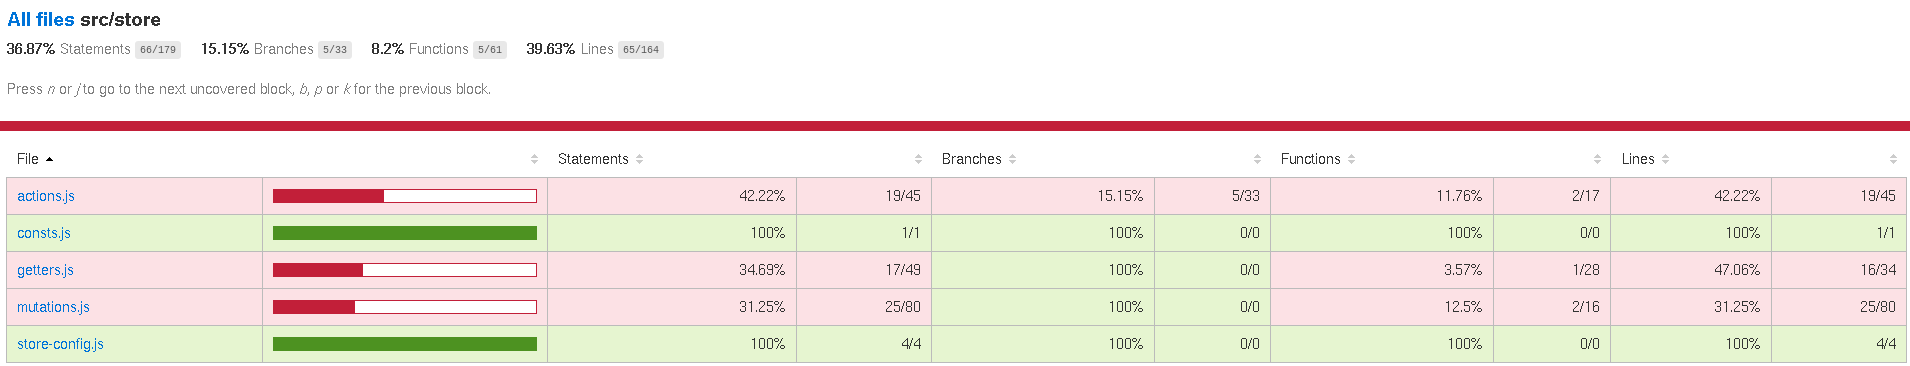
\includegraphics[scale=0.25]{cobertura}
	\caption{Cobertura calculada por \textit{jest} (no real).}\label{fig:cobertura}
\end{figure}

	\begin{table}
	\centering
	\begin{tabular}{p{1cm}p{3cm}p{10cm}p{1.5cm}}
		\toprule
		ID & Prueba & Descripci�n & \textit{Action} \\ \midrule
		PU-1 & A�adir terna &  A�ade una terna al grafo y comprueba que el n�mero total de ternas de este se ha incrementado en uno. & ACC-1 \\ \midrule
		PU-2 & Eliminar ternas seg�n recurso & Elimina todas las ternas que tengan el recurso ``Analista'' en cualquiera de sus posiciones; se cuentan las ternas eliminadas y se comprueba que el tama�o final del grafo es correcto. & ACC-2 \\ \midrule
		PU-3 & Editar recurso &  Se edita el recurso ``Analista'' cambi�ndolo por otro nombre y se recuperan las ternas asociadas al antiguo y nuevo recurso antes y despu�s de su edici�n, comprobando que el n�mero de ternas asociadas es el correcto en cada caso. & ACC-3 \\ \midrule
		PU-4 & Editar literal  & Se comprueba que, tras editar el literal asociado a un objeto de una terna recuperada, el contenido de este cambia en consecuencia. & ACC-5 \\ \midrule
		PU-5 & A�adir literal &  A�ade un literal como propiedad de un recurso y se comprueba que el n�mero de propiedades de tipo literal para ese recurso se incrementa en uno. & ACC-6 \\ \midrule
		PU-6 & Importar N3 & Se incluye cadena de texto simulando un fichero en formato Turtle, se importa y se comprueba que el n�mero de ternas del grafo coincide con las importadas. & ACC-7 \\ \midrule
		PU-7 & A�adir N3 & Se incluye cadena de texto simulando un fichero en formato Turtle, se a�ade al grafo actual y se comprueba que el n�mero de ternas del grafo resultante es la suma de las que ten�a anteriormente m�s las importadas. & ACC-8 \\ \midrule
		PU-8 & Eliminar N3 & Se incluye cadena de texto simulando un fichero en formato Turtle, se a�aden las ternas al grafo, se cuenta el n�mero total de ternas, se eliminan de nuevo del grafo actual y se comprueba que el n�mero de ternas del grafo resultante es el original. & ACC-9 \\ \midrule
		PU-9 & Importar actividad & Se importa una actividad en formato \textit{Markdown} y se comprueba que la variable de estado que aloja su contenido deja de estar vac�a. & ACC-10 \\ \midrule
		PU-10 & Cargar vocabulario & Se verifica que el cambio de estado de un vocabulario de inactivo a activo ocurre, consultando el mismo tras la operaci�n. & ACC-13 \\ 
		\bottomrule
	\end{tabular}
\caption{Listado de pruebas unitarias de actions}\label{tab:test-actions}
\end{table}

	\begin{table}
	\centering
	\begin{tabular}{p{1.2cm}p{5cm}p{8cm}p{1.2cm}}		
		\toprule
		ID & Prueba & Descripci�n & \textit{Getter} \\ \midrule
		PU-11 & Recuperar listado de sujetos por predicado y objeto & Se recuperan todos los sujetos de tipo owl:Class y se comprueba que el n�mero devuelto es correcto. & GET-1\\ \midrule
		PU-12 & Recuperar listado de sujetos por predicado & Se recupera una lista de sujetos de tipo anotaci�n, por ejemplo, y se comprueba que se devuelve el n�mero de correcto de resultados. & GET-2 \\ \midrule
		PU-13 & Recuperar listado de objetos por predicado y sujeto & Se recuperan todos los objetos para el sujeto ``Analista'' y el predicado etiqueta, y se comprueba que el n�mero devuelvo es el correcto.  &GET-3 \\ \midrule
		PU-14 & Recuperar listado de ternas para un sujeto dado & Se recupera un listado de ternas para el sujeto ``Analista'' y se comprueba que el n�mero devuelto es el correcto. & GET-4 \\ \midrule
		PU-15 & Recuperar listado de ternas para un objeto dado & Se recupera un listado de ternas cuyo objeto es owl:Class y se comprueba que el n�mero resultante es el correcto. & GET-5 \\ \midrule
		PU-16 & Recuperar listado de todas las ternas del almac�n & Se recuperan todas las ternas y se comprueba que el resultado es el n�mero total de ternas cargadas en el grafo. & GET-6 \\ \midrule
		PU-17 & Recuperar listado de todas las propiedades cargadas por defecto & Se recupera el listado de todas las propiedades cargadas por defecto en la aplicaci�n y se comprueba que el n�mero total resultante es el correcto. & GET-7 \\ 
		\bottomrule
	\end{tabular}
	\caption{Listado de pruebas unitarias de getters}\label{tab:test-getters}
\end{table}

\pagebreak

\subsection{Pruebas extremo a extremo (\textit{end-to-end})}

Las pruebas extremo a extremo (o \textit{end-to-end}) permiten probar la interfaz de usuario a trav�s de un navegador automatizado. En su forma m�s b�sica, este tipo de pruebas permite comprobar la existencia de determinados elementos en el DOM\footnote{Document Object Model} de la aplicaci�n web, as� como verificar que su contenido es correcto.

Para el presente proyecto se ha optado por codificar una prueba extremo a extremo por cada m�dulo definido en la secci�n \ref{sec:arquitectura-de-m�dulos}, a modo de \textit{sanity check} o prueba de cordura. En el cuadro \ref{tab:test-e2e} se detalla un listado de los mismos relacionados con sus correspondientes m�dulos:

\vspace*{\baselineskip}
\vspace*{\baselineskip}

	\begin{table}[htb]
	\centering
	\begin{tabular}{p{2cm}p{3cm}p{8cm}p{2cm}}		
		\toprule
		ID & Prueba  & Descripci�n & M�dulo \\ \midrule
		E2E-1 & Actividad & Se comprueba n�mero de \textit{inputs} y el contenido de p�rrafo. & MOD-1\\ \midrule
		E2E-2 & Vocabulario & Se comprueba n�mero de \textit{inputs} y el contenido de una cabecera. & MOD-2 \\ \midrule
		E2E-3 & Importar/exportar & Se comprueba n�mero de botones y el contenido de una cabecera.  & MOD-3 \\ \midrule
		E2E-4 & Modelado & Se comprueba el n�mero de enlaces y el contenido de una pesta�a. & MOD-4 \\ \midrule
		E2E-5 & Poblamiento & Se comprueba el n�mero de \textit{inputs} y una cabecera. & MOD-5 \\ \midrule
		E2E-6 & Consulta & Se comprueba el contenido de una etiqueta y el n�mero de \textit{textarea}. & MOD-6 \\ 
		\bottomrule
	\end{tabular}
	\caption{Listado de pruebas extremo a extremo.}\label{tab:test-e2e}
\end{table}
\cleardoublepage{}

\chapter{Resultados}

<....>\cleardoublepage{}

\chapter{Conclusiones y l�neas de trabajo futuras}


\section{Conclusiones}

Alimentar la Web con datos estructurados y contextualizados con metadatos no ha de ser una labor exclusiva de entornos acad�micos y universitarios. Si bien son estas organizaciones las que han modelado dominios de informaci�n y liberado conjuntos de datos de forma masiva a lo largo de los �ltimos a�os, es necesario extender esta responsabilidad a otros organismos p�blicos y privados y, por qu� no, a potenciales usuarios o clientes particulares. Solo a partir de ese momento, el relato inicial de Berners-Lee\cite{bernerslee01} en su primera definici�n de la Web Sem�ntica ser� una realidad en nuestra Sociedad.

No obstante, a�n queda mucho trabajo por hacer. Organizaciones p�blicas y privadas han de concienciarse de la enorme importancia de poner a disposici�n de la Sociedad en general datos estructurados en formatos reutilizables. S�lo de esta forma crecer� el inter�s en su tratamiento y explotaci�n, as� como en el desarrollo de agentes inteligentes que sean capaz de procesarlos para generar nuevos resultados de an�lisis. No hay m�s que recurrir a los datos del Estudio de Caracterizaci�n del Sector Infomediario en Espa�a\cite{ontsi01} proporcionados por el Observatorio Nacional de las Telecomunicaciones y de la Sociedad de la Informaci�n, que recogen que el 70\% de las empresas encuestadas accede a datos no estructurados, frente al 69\% que lo hace a datos en formatos abiertos (si bien no se especifica si se trata de datos a nivel de datos abiertos enlazados o \textit{linked open data}).

La comunidad de tecnol�gos y desarrolladores de aplicaciones para la Web Sem�ntica debe trabajar por la democratizaci�n de esta tecnolog�a. Con los niveles de complejidad conceptual y de uso actuales, su difusi�n entre el p�blico general se hace complicada. En este sentido, las grandes revoluciones surgidas en torno al mundo del desarrollo de \textit{frontend} web en general (y \textit{Javascript} en particular) y el nivel de madurez alcanzado en estos momentos por las tecnolog�as de la Web Sem�ntica, favorecen la llegada del momento m�s propicio en los �ltimos veinte a�os para lograr un impulso real. A�n son pocas las comunidades de desarrolladores trabajando en ofrecer servicios sem�nticos a trav�s de \textit{Javascript}, pero la existencia de un \textit{``community group''}\cite{rdfw3ccg} que aglutina esfuerzos para aunar a dichas comunidades en un s�lo proyecto es una noticia prometedora de cara al futuro de esta tecnolog�a.

Como peque�a contribuci�n a estos esfuerzos de difusi�n y democratizaci�n, se ha desarrollado el presente proyecto, que representa la culminaci�n de meses de trabajo pero tambi�n el inicio de la vida de un producto. Se sientan las bases para obtener una herramienta acad�mica que permita acercar las tecnolog�as de la Web Sem�ntica a cualquier no iniciado. Si bien en esta primera versi�n ya se cuenta con una aplicaci�n funcional, el estado de las bibliotecas que integra y las posibilidades de RDF y SPARQL sugieren unas expectativas de evoluci�n lo suficientemente optimistas como para continuar su desarrollo y no abandonar su mantenimiento.

A partir de este punto, la hoja de ruta que se propone para el producto desarrollado en el presente proyecto es clara: en un primer curso acad�mico, comenzar a utilizarlo a modo de prueba piloto en asignaturas t�cnicas relacionadas con la Web Sem�ntica a trav�s de actividades opcionales (para mejorar la nota total del alumno, por ejemplo) e ir evaluando su idoneidad de cara a su manejo en el entorno para el que fue pensado. Paralelamente, la aplicaci�n puede seguir siendo mejorada y perfeccionada, en caso de aparici�n de defectos inesperados (algo, por otra parte, perfectamente asumible hoy en d�a).

Un claro compromiso por parte del autor del proyecto debe ser para con la Comunidad Educativa, y especialmente para los grupos de trabajo como el \textit{RDF Javascript Libraries Community Group} por su inestimable ayuda prestada. Por tanto, parece razonable trabajar en una futura traducci�n al idioma ingl�s para permitir su publicaci�n como repositorio de c�digo abierto y revertir el desarrollo a la Comunidad.

No se podr�a concluir este cap�tulo de conclusiones sin valorar las competencias tecnol�gicas y organizativas que el desarrollo del proyecto ha permitido adquirir a su autor: profundizaci�n en el modelado RDF, las arquitecturas de aplicaciones de la Web Sem�ntica, los motores de consultas SPARQL y el desarrollo en marcos de trabajo \textit{Javascript} completos y bien estructurados como Vue.js (una inversi�n, esta �ltima, m�s que rentable en t�rminos de utilizaci�n de la tecnolog�a).

Tomar decisiones entre altas dosis de incertidumbre no es sencillo, y menos a�n cuando la oferta tecnol�gica es numerosa y variada (como es el caso, por ejemplo, de las bibliotecas de componentes gr�ficos para Vue). Adem�s, la complejidad inicial del desarrollo en \textit{Javascript} no presenta una curva de aprendizaje suave, especialmente en la configuraci�n del entorno necesario: empaquetadores, \textit{``transpilers''} con sus m�dulos asociados, existencia de diversos est�ndares conviviendo entre distintos m�dulos que complican su integraci�n, etc.

Por otra parte, los trabajos previos de implementaci�n de RDF en \textit{Javascript} tambi�n son numerosos y confusos (prueba de ello es la reciente noticia de Junio de este mismo a�o, 2018, indicando la unificaci�n de las diferentes implementaciones existentes en una �nica implementaci�n). Afortunadamente, la ayuda y los consejos de los propios desarrolladores, ya con experiencia, ha permitido enfocar el proyecto con las estrategias adecuadas.

En resumidas cuentas, se ha tratado de obtener un producto apto para la formaci�n acad�mica en tecnolog�as de la Web Sem�ntica, cumpliendo razonablemente con los objetivos iniciales y abriendo un camino al desarrollo de una herramienta mucho m�s completa que pueda aprovecharse de las tecnolog�as emergentes en el �rea del \textit{frontend} web. Se han utilizado bibliotecas y m�dulos est�ndares dentro de la situaci�n actual, lo que permitir� una mayor facilidad de mantenimiento en el futuro y pretende abrir el camino a evoluciones m�s ambiciosas. A fecha de finalizaci�n de la presente memoria, ya se est�n manteniendo conversaciones con el Director del Proyecto para el futuro uso de la aplicaci�n en la actividad docente, lo que permitir�, sin duda, obtener \textit{feedback} de cara a su futura mejora. El tablero Kanban del proyecto y el propio repositorio en Github est�n disponibles desde este momento para incorporar nuevas tarjetas y peticiones de evoluci�n o mejora.

\section{L�neas de trabajo futuras}

Como punto de partida para futuras mejoras y nuevas funcionalidades, se proponen las siguientes l�neas de trabajo:

\begin{itemize}
\item Integrar la primera versi�n estable (una vez publicada) de los distintos m�dulos de la plataforma Comunica y optimizar el uso de dependencias.
\item Integrar las futuras versiones del marco de trabajo de componentes Vuetify y utilizar nuevos componentes como la estructura jer�rquica (en �rbol) para representar clases y propiedades.
\item Integrar o desarrollar consultas SPARQL con Comunica a grafos en RDFXML\footnote{\url{https://github.com/comunica/comunica/issues/140}}
\item Incrementar la cobertura de pruebas unitarias y extremo a extremo
\item Re-orientar las operaciones de consulta a trav�s del m�dulo \textit{actor-init-sparql-rdfjs} (ver secci�n \ref{sec:motor-de-consultas-en-el-proyecto})
\item Funcionalidad de exportar a un formato JSON-raw (una lista de objetos con ternas).
\item Posibilidad de modificar los prefijos a incluir en las consultas. En general, facilitar el uso de prefijos.
\item Enriquecer y refactorizar la funcionalidad de modelado.
\item Soportar m�ltiples grafos.
\item Revisar la carga de t�rminos b�sicos y estudiar la viabilidad de carga en l�nea desde una ontolog�a est�ndar.
\item Traducci�n de la aplicaci�n al idioma ingl�s y puesta a disposici�n de las distintas comunidades de desarrolladores y usuarios.
\end{itemize} 




\cleardoublepage{}

\bibliographystyle{unsrt}
\bibliography{biblio/biblio-pfg}


\appendix
\cleardoublepage{}\renewcommand{\appendixname}{Anexo}

\chapter{Manual de usuario}

El manual de usuario forma parte de la propia aplicaci�n web, pudiendo ser accedido a trav�s del enlace ``Ayuda'' ubicado en el pie de p�gina de la misma.



\end{document}
